%%%%%%%%%%%%%%%%%%%%%%%%%%%%%%%%%%%%%%%%%%%%%%%%%%%%%%%%%%
% # Self-Paced Reading Experiment
%%%%%%%%%%%%%%%%%%%%%%%%%%%%%%%%%%%%%%%%%%%%%%%%%%%%%%%%%%

\chapter{Self-Paced Reading Experiment}\label{ch-spr}

This chapter reports on the self-paced reading task (SPRT), which probed the processing of gapped vs. resumptive RCs during real-time sentence comprehension, focusing on the same three relativization environments as in the EPT. I begin in Section~\ref{spr-rq} by listing the research questions (RQs) that guided the creation of this task. I describe the design of the task in Section~\ref{spr-design} and the data analysis procedures in Section~\ref{spr-analysis}. In Sections \ref{spr-rt}--\ref{spr-qrt-proficiency}, I walk the reader through the results, attending to each of the RQs in turn and drawing on both response-time (RT) data and comprehension-question accuracy data. For each analysis, I present the results from the ORC study followed by the results from the SRC study. Section~\ref{spr-conclusion} concludes the chapter.

%========================================================%
\section{Research questions}\label{spr-rq}
%========================================================%

There are four main RQs for the SPRT, all of which pertain to the real-time comprehension of L1 and/or L2 English RCs:

\begin{enumerate}[\bfseries RQ1:,itemsep=5pt]
\item {\bfseries How does resumption affect RTs at the regions of interest?}\par\nobreak
Prediction: RTs following RPs will be faster than RTs following gaps in conditions that are difficult for relativization. This would constitute preliminary evidence that resumption eases real-time comprehension of RCs when there is strain on the processor.
\end{enumerate}\vspace{5pt}

\begin{enumerate}[\bfseries RQ2:,itemsep=5pt]
\item {\bfseries How does resumption affect comprehension-question accuracy?}\par\nobreak
Prediction: Accuracy on comprehension questions will be higher for RP trials than for gap trials, at least in conditions that are difficult for relativization. Such a pattern of results would provide corroborating evidence that resumption facilitates RC comprehension under processing strain.
\end{enumerate}\vspace{5pt}

\begin{enumerate}[\bfseries RQ3:,itemsep=5pt]
\item {\bfseries How does resumption affect RTs for comprehension questions?}\par\nobreak
Prediction: RTs for comprehension questions (henceforth, comprehension-question RTs) will be faster in RP trials than in gap trials, at least in conditions that put strain on the processor. This result would also be consistent with resumption making RCs easier to comprehend when processing load is high.
\end{enumerate}\vspace{5pt}

\begin{enumerate}[\bfseries RQ4:,itemsep=5pt]
\item {\bfseries How does L2 proficiency affect the data patterns?}\par\nobreak
Prediction: Any processing advantage for RPs over gaps will become less pronounced as L2 proficiency increases, at least in RC environments where English allows gapping. Such a pattern of results would suggest that higher levels of L2 English proficiency are associated with (a)~more efficient RC processing and/or (b)~increased sensitivity to the English prohibition on resumption in RCs.
\end{enumerate}

%========================================================%
\section{Design and procedure}\label{spr-design}
%========================================================%

The ORC and SRC versions of the task shared the same 2~×~3 factorial design crossing dependency type (\textsc{dependency}: gap vs. RP) and syntactic environment (\textsc{environment}: short-distance vs. long-distance vs. \textit{wh}-island), as shown in Tables \ref{tab:spr-cond-orc} and \ref{tab:spr-cond-src}. The two levels of the \textsc{dependency} factor will henceforth be referred to as the `Gap' and `RP' conditions, and the three levels of the \textsc{environment} factor will henceforth be referred to as the `Short,' `Long,' and `Island' conditions.  Each version of the task had 30 critical items (6 conditions × 5 tokens, Latin-squared) and 42 fillers. The presentation order for critical and filler items was pseudorandomized so that no two critical items appeared consecutively. The full list of critical and filler stimuli is provided in Appendix \ref{app-materials-spr}.

\begin{table}
\caption{Critical conditions in the ORC self-paced reading task}\label{tab:spr-cond-orc}
\raggedright\setstretch{1}
\begin{tabularx}{\linewidth}{lL}\toprule
Environment~~~~ & Example stimulus in the Gap and RP conditions \\\midrule
Short & I think Mary knows the man that these detectives arrested \{\_\_/*him\} \newline \myuline{at} \myuline{the} \myuline{beginning} of the week. \\
Long & Mary knows the man that I think these detectives arrested \{\_\_/*him\} \newline \myuline{at} \myuline{the} \myuline{beginning} of the week. \\
Island & Mary knows the man that I wonder which detectives arrested \{*\_\_/*him\} \newline \myuline{at} \myuline{the} \myuline{beginning} of the week. \\\bottomrule
\end{tabularx}
\textit{Note}. Underlining indicates regions of interest.
\vspace{-12pt}
\end{table}

\begin{table}
\caption{Critical conditions in the SRC self-paced reading task}\label{tab:spr-cond-src}
\raggedright\setstretch{1}
\begin{tabularx}{\linewidth}{lL}\toprule
Environment~~~~ & Example stimulus in the Gap and RP conditions \\\midrule
Short & I think Mary knows the man that \{\_\_/*he\} \myuline{borrowed} \myuline{this} \myuline{book} at the \newline beginning of the month. \\
Long & Mary knows the man that I think \{\_\_/*he\} \myuline{borrowed} \myuline{this} \myuline{book} at the \newline beginning of the month. \\
Island & Mary knows the man that I wonder which book \{*\_\_/*he\} \myuline{borrowed} \myuline{at} \myuline{the} \newline beginning of the month. \\\bottomrule
\end{tabularx}
\textit{Note}. Underlining indicates regions of interest.
\vspace{-12pt}
\end{table}

The regions of interest were the three words following the gap or the RP. \textcite{hofmeister.norcliffe2013} used the two words following the gap/RP as the regions of interest in their L1-English study, but I decided to extend this to three words because processing effects are sometimes delayed in L2ers relative to native speakers (\cite{keating2009}, p.~527; \cite{lim.christianson2015}, p.~1301; \cite{sabourin.stowe2008}, p.~425; \cite{song2015}, p.~257). 

The fillers were designed to be similar to the critical items in both length and complexity. As Table \ref{tab:spr-filler} shows, there were four sentence types (F1--F4) used in the fillers (all with short-distance ORCs/SRCs in triclausal sentences): Two of these had both grammatical (G) and ungrammatical (U) variants, whereas the remaining two sentence types were all grammatical. There were 42 fillers in total---seven each of F1G, F1U, F2G, F2U, F3G, and F4G---yielding a 1:1 ratio of expected-to-be acceptable trials to expected-to-be unacceptable trails (at least for ENSs) across all critical and filler items encountered by each participant. The F1U and F2U fillers were similar in formulation to their grammatical counterparts except that something had been added or removed from the sentence, thereby rendering it ill-formed. Ungrammaticality was induced in the F1U fillers by adding an overt direct object to a short passive and in the F2U fillers by deleting an obligatory determiner preceding a singular count noun. I made a point of including the verb \textit{wonder} in the F3G fillers so that participants would not encounter that verb solely in Island-condition critical sentences, which were expected to be unacceptable, at least for ENSs, regardless of whether an RP was present.

\begin{table}
\caption{Filler types in the ORC and SRC self-paced reading tasks}\label{tab:spr-filler}
\raggedright\setstretch{1}
\begin{tabularx}{\linewidth}{lL}\toprule
Type & \phantom{* }Stimulus \\\midrule
F1G & \phantom{* }Mary says this man saw the criminals that attacked me at the beginning of the week. \\
F1U & * This woman says John met the protesters that were criticized me at the end of the week. \\
F2G & \phantom{* }This man says Tina found the article that I published at the end of the year. \\
F2U & * Mike says this woman likes essay that I published at the beginning of the year. \\
F3G & \phantom{* }This woman wonders who saw the journalists that teased Bill at the end of the month. \\
F4G & \phantom{* }Anna thinks this man likes the story that she told at the end of the night. \\\bottomrule
\end{tabularx}
\vspace{-12pt}
\end{table}

The stimulus sentences were presented in word-by-word fashion on a computer screen in moving-window format (\cite{just.etal1982}), as shown in Figure~\ref{fig:spr-trial}.

\begin{figure}
\caption{In-progress trial in the SRC self-paced reading task} \label{fig:spr-trial}
\raggedright\setstretch{1}
\fbox{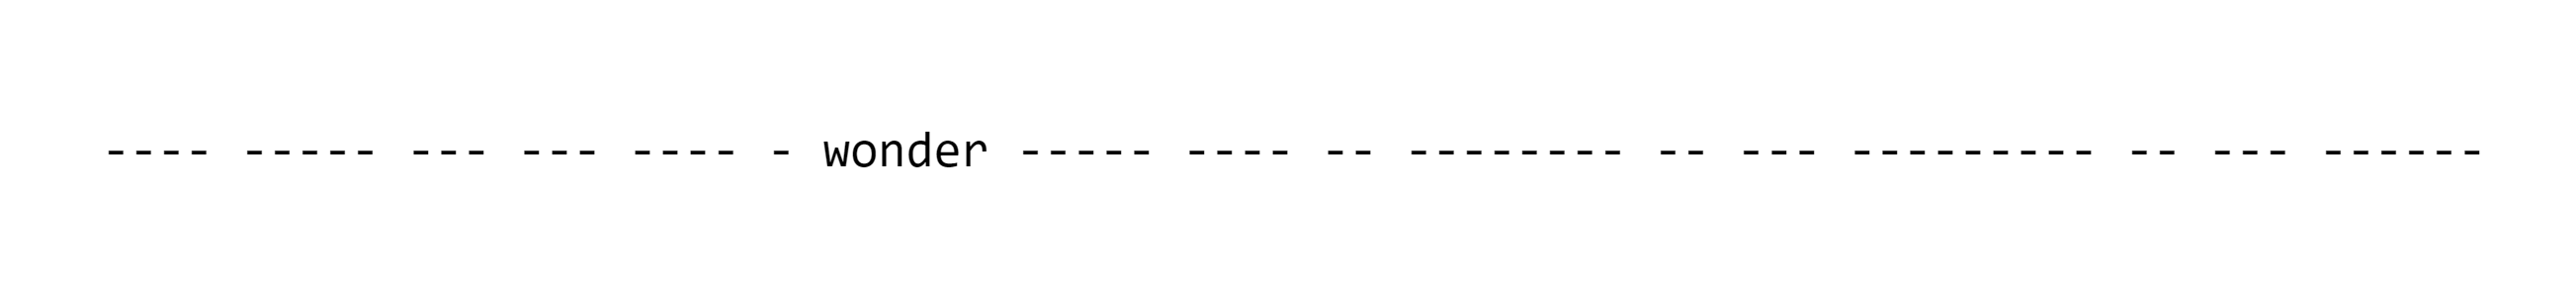
\includegraphics[width=\textwidth]{../image/spr-trial-src.png}}
\textit{Note}. Stimulus shown in the SRC [RP + Island] condition with the seventh word exposed.
\vspace{-12pt}
\end{figure}

\noindent Each stimulus was displayed as a single line of text, and participants pressed the space bar to advance through the sentence. If the reading speed for a sentence was less than, on average, 200 ms per word, a message would appear on the screen for three seconds asking the participant to read more carefully; this message was presented in the participant's native language to ensure comprehension. RTs for the reading of each word were logged for later analysis.

A comprehension question in multiple-choice format followed each stimulus. The purpose of these questions was twofold: (a)~to ensure that participants were reading the sentences for meaning and (b)~to test whether they correctly associated the gap/RP with the head of the RC (see~\cite{morgan.etal2020}, p.~3; Section~\ref{res-morgan}). For critical trials, correctly answering the question relied on accurate dependency resolution, as demonstrated in Figure \ref{fig:spr-question}, which is the comprehension question for the stimulus sentences in Table \ref{tab:spr-cond-src} (e.g.,~\textit{Mary knows the man that I wonder which book he borrowed at the beginning of the month} in the SRC study's [RP + Island] condition). Each comprehension question had two blanks to fill in, and participants had to select the correct option for both blanks for their answer to be scored as correct (otherwise, it was scored as incorrect); in critical trials, that meant correctly identifying the subject and direct object of the verb in the clause containing the gap/RP.

\begin{figure}
\caption{Comprehension question for a critical trial in the SRC self-paced reading task} \label{fig:spr-question}
\raggedright\setstretch{1}
\fbox{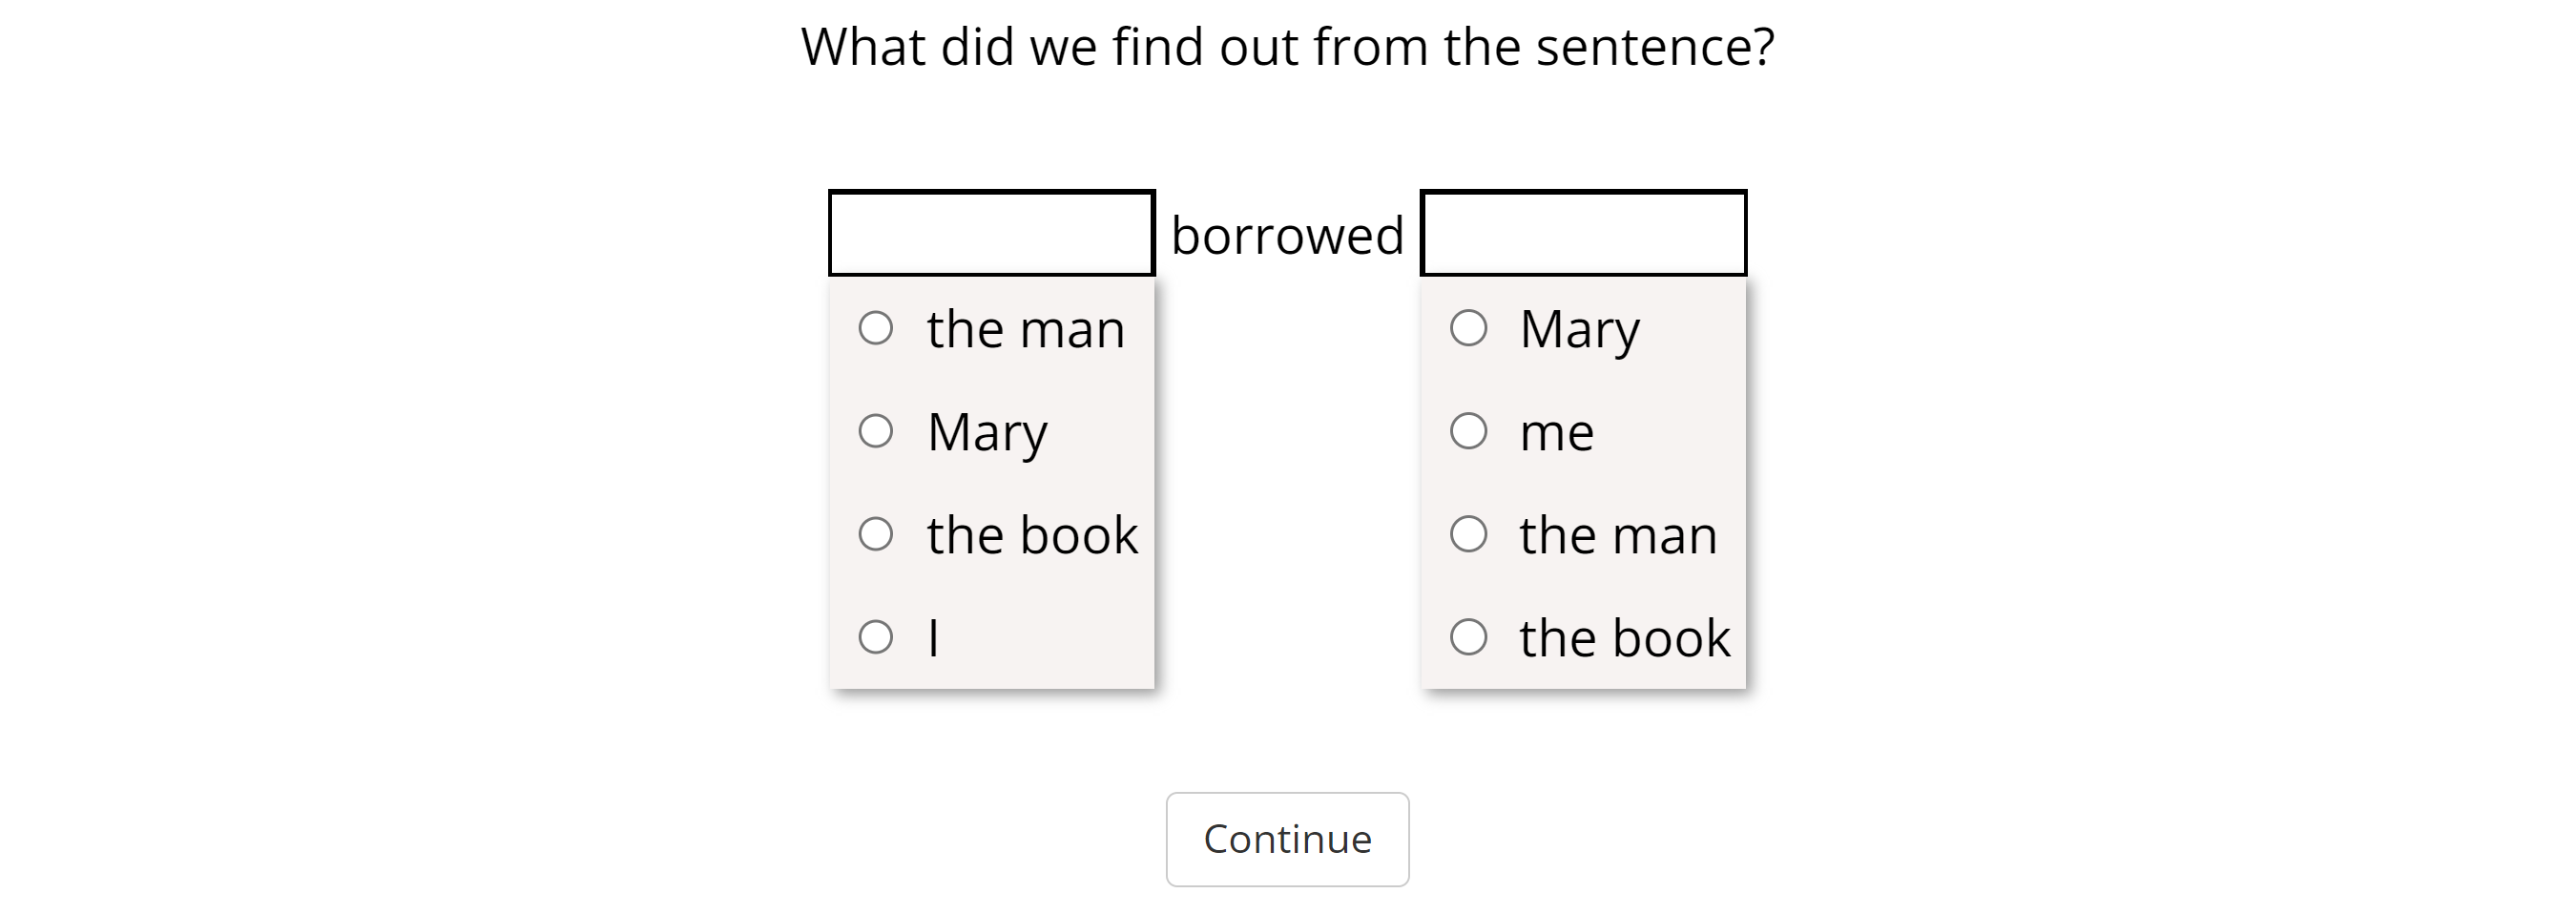
\includegraphics[width=.99\textwidth]{../image/spr-question-src-2.png}}
\textit{Note}. Correct answer: \myuline{the man} borrowed \myuline{the book}.
\vspace{-12pt}
\end{figure}

\noindent Comprehension questions for fillers targeted information in different parts of the sentence to discourage participants from developing answer strategies that do not rely on a genuine understanding of the sentence. Responses and RTs (to read and respond to the question) were both recorded so that they could be analyzed later. The order of the multiple-choice options was randomized across trials, and the experiment automatically notified participants when their responses were incorrect. 

After reading the instructions, participants completed three practice items meant to familiarize them with the experimental procedure before they started the main portion of the task. They had to answer all three practice items correctly to proceed. Participants who made errors were automatically sent back to the instructions page. The questions were the same each time the participant entered the practice phase of the task, but with the presentation order randomized. The instructions, practice items, and warning messages can be found in Appendix \ref{app-materials-spr}.

%========================================================%
\section{Data processing and analysis}\label{spr-analysis}
%========================================================%

Nine participants were lost from the SPRT data due to experimental error: one KLE in the ORC study (1/69~=~1\%), four MLEs in the ORC study (4/76~=~5\%), and four MLEs in the SRC study (4/73~=~5\%). A further four participants were flagged as outliers and removed for having an accuracy rate more than three standard deviations below the group mean on comprehension questions for both critical and filler trials (calculated separately): in the ORC study, one KLE (1/69 = 1\%) and two MLEs (2/76 = 3\%); in the SRC study, one KLE (1/66 = 2\%). This left 227 participants for the ORC analyses (90 ENSs, 67 KLEs, and 70 MLEs) and 195 participants for the SRC analyses (61 ENSs, 65 KLEs, and 69 MLEs).

Following standard data-cleaning procedures for SPRTs (see~\cite{hammerly2022}; \cite{hofmeister2011}; \cite{jackson2010}; \cite{mifka-profozic.etal2020}; \cite{morgan.etal2020}; \cite{santi.etal2019}), RTs faster than 100 ms or slower than 6,000 ms were interpreted as momentary lapses in attention and excluded. This lead to the removal of 0.22\% of the critical-trial ORC data (ENS: 0.11\%; KLE: 0.27\%; MLE: 0.31\%) and 0.29\% of the critical-trial SRC data (ENS: 0.31\%; KLE: 0.25\%; MLE: 0.31\%). RTs that deviated by more than two standard deviations from the mean for each \textsc{dependency × environment × group × region} combination were also removed (see~\cite{hofmeister2011}; \cite{hofmeister.norcliffe2013}; \cite{jackson2010}; \cite{mifka-profozic.etal2020}; \cite{santi.etal2019}), affecting 3.87\% of the remaining critical-trial ORC data (ENS: 3.10\%; KLE: 4.27\%; MLE: 4.47\%) and 4.03\% of the remaining critical-trial SRC data (ENS: 3.02\%; KLE: 4.25\%; MLE 4.71\%).

RTs were normalized via a log transformation (see~\cite{hofmeister2011}; \cite{hofmeister.norcliffe2013}; \cite{mifka-profozic.etal2020}; \cite{santi.etal2019}) and analyzed with separate linear mixed-effects models for each region of interest (see~\cite{hofmeister2011}; \cite{hwang.schafer2009}; \cite{jackson2010}; \cite{keating.jegerski2015}). The models had fixed effects for \textsc{dependency}, \textsc{environment}, and \textsc{group} and random effects for \textsc{participant} and \textsc{item}.

My prediction was that when there is strain on the processor (i.e.,~in more complex syntactic environments), RTs would be faster after RPs than after gaps at one or more of the regions of interest (\cite{hammerly2022}; \cite{hofmeister.norcliffe2013}). Such a result would suggest that RPs facilitate RC comprehension. In RTs for all groups in the Island condition and for L2ers perhaps also in the Long condition, I expected that dependency resolution would be sufficiently difficult to evince a significant RP-over-gap advantage. I further predicted that as the amount of strain on the processor is reduced, the size of the processing advantage conferred by RPs would shrink to the point of vanishing entirely. On the other hand, in environments where it is particularly easy to resolve the RC dependency with a gap before arriving at the RP, I reasoned that the RP might in fact trigger a surprisal effect strong enough to cause a slowdown in RP-trial RTs relative to gap-trial RTs (\cite{hammerly2022}, p.~828). I anticipated that gapped dependency resolution would be easy enough for this surprisal effect to be observed only in the Short condition, and only for ENSs.

For the comprehension-question data, the binary accuracy scores were analyzed using a mixed-effects logistic regression model and the RTs were analyzed using a linear mixed-effects regression model. These models both had fixed effects for \textsc{dependency}, \textsc{environment}, and \textsc{group} and random effects for \textsc{participant} and \textsc{item}. In environments that put strain on the processor, I expected that (a) accuracy rates would be higher with RPs than with gaps and (b) RTs would be faster with RPs than with gaps. Such a pattern of results would show that participants accurately resolved the resumptive RC dependencies and would provide further evidence that RPs facilitate RC comprehension under processing strain.

Data cleaning for comprehension-question RTs followed the same procedure as for region-of-interest RTs, except that the upper limit for the absolute cutoffs was adjusted from 3,000~ms (3~seconds) to 30,000~ms (30~seconds). Absolute-cutoff-based trimming led to the exclusion of 0.82\% of the critical-trial ORC data (ENS: 0.41\%; KLE: 0.85\%; MLE: 1.33\%) and 1.40\% of the critical-trial SRC data (ENS: 1.09\%; KLE: 0.67\%; MLE: 2.37\%). Additional trimming with a cutoff of two standard deviations from the mean for each \textsc{dependency × environment × group × region} combination resulted in the removal of 5.14\% of the remaining critical-trial ORC data (ENS: 5.36\%; KLE: 4.92\%; MLE: 5.07\%) and 4.91\% of the remaining critical-trial SRC data (ENS: 4.92\%; KLE: 4.54\%; MLE: 5.24\%).

Finally, to test for L2 proficiency effects, I reanalyzed the region-of-interest RT data, the comprehension-question accuracy data, and the comprehension-question RT data for the L2ers, adding \textsc{proficiency} to each model as a continuous fixed effect. I reasoned that if processing becomes more efficient as proficiency increases, there should be a negative relationship between \textsc{proficiency} and the magnitude of any RP facilitation effects detected in the main analyses, at least in environments where gapping is permitted in English.

Assuming, following the literature, that the Mandarin translations of the stimuli are grammatical with RPs in at least the SRC Long condition, the SRC Island condition, and all the ORC conditions (as~my Mandarin language consultants likewise led me to believe), I also expected that MLEs would be less likely than ENSs and KLEs to experience surprisal upon encountering RPs. I therefore reasoned that the MLE group would, if anything, have even larger processing facilitation effects associated with RPs than the other participant groups.

%========================================================%
\section{RTs at the regions of interest}\label{spr-rt}
%========================================================%

First, let us consider RQ1, which asks how resumption affects RTs at the regions of interest. Figures \ref{fig:spr-logrt-orc} and \ref{fig:spr-logrt-src} show the mean log RTs at the regions of interest for, respectively, the ORC dataset and the SRC dataset. Plots of the raw RT data, which displayed the same general pattern of results, are provided in Appendix~\ref{app-results-spr}, Figures~\ref{fig:app-orc-spr-rt} and \ref{fig:app-src-spr-rt}.

\begin{figure}
\caption{Mean log RTs at the regions of interest in the ORC self-paced reading task} \label{fig:spr-logrt-orc}
\raggedright\setstretch{1}
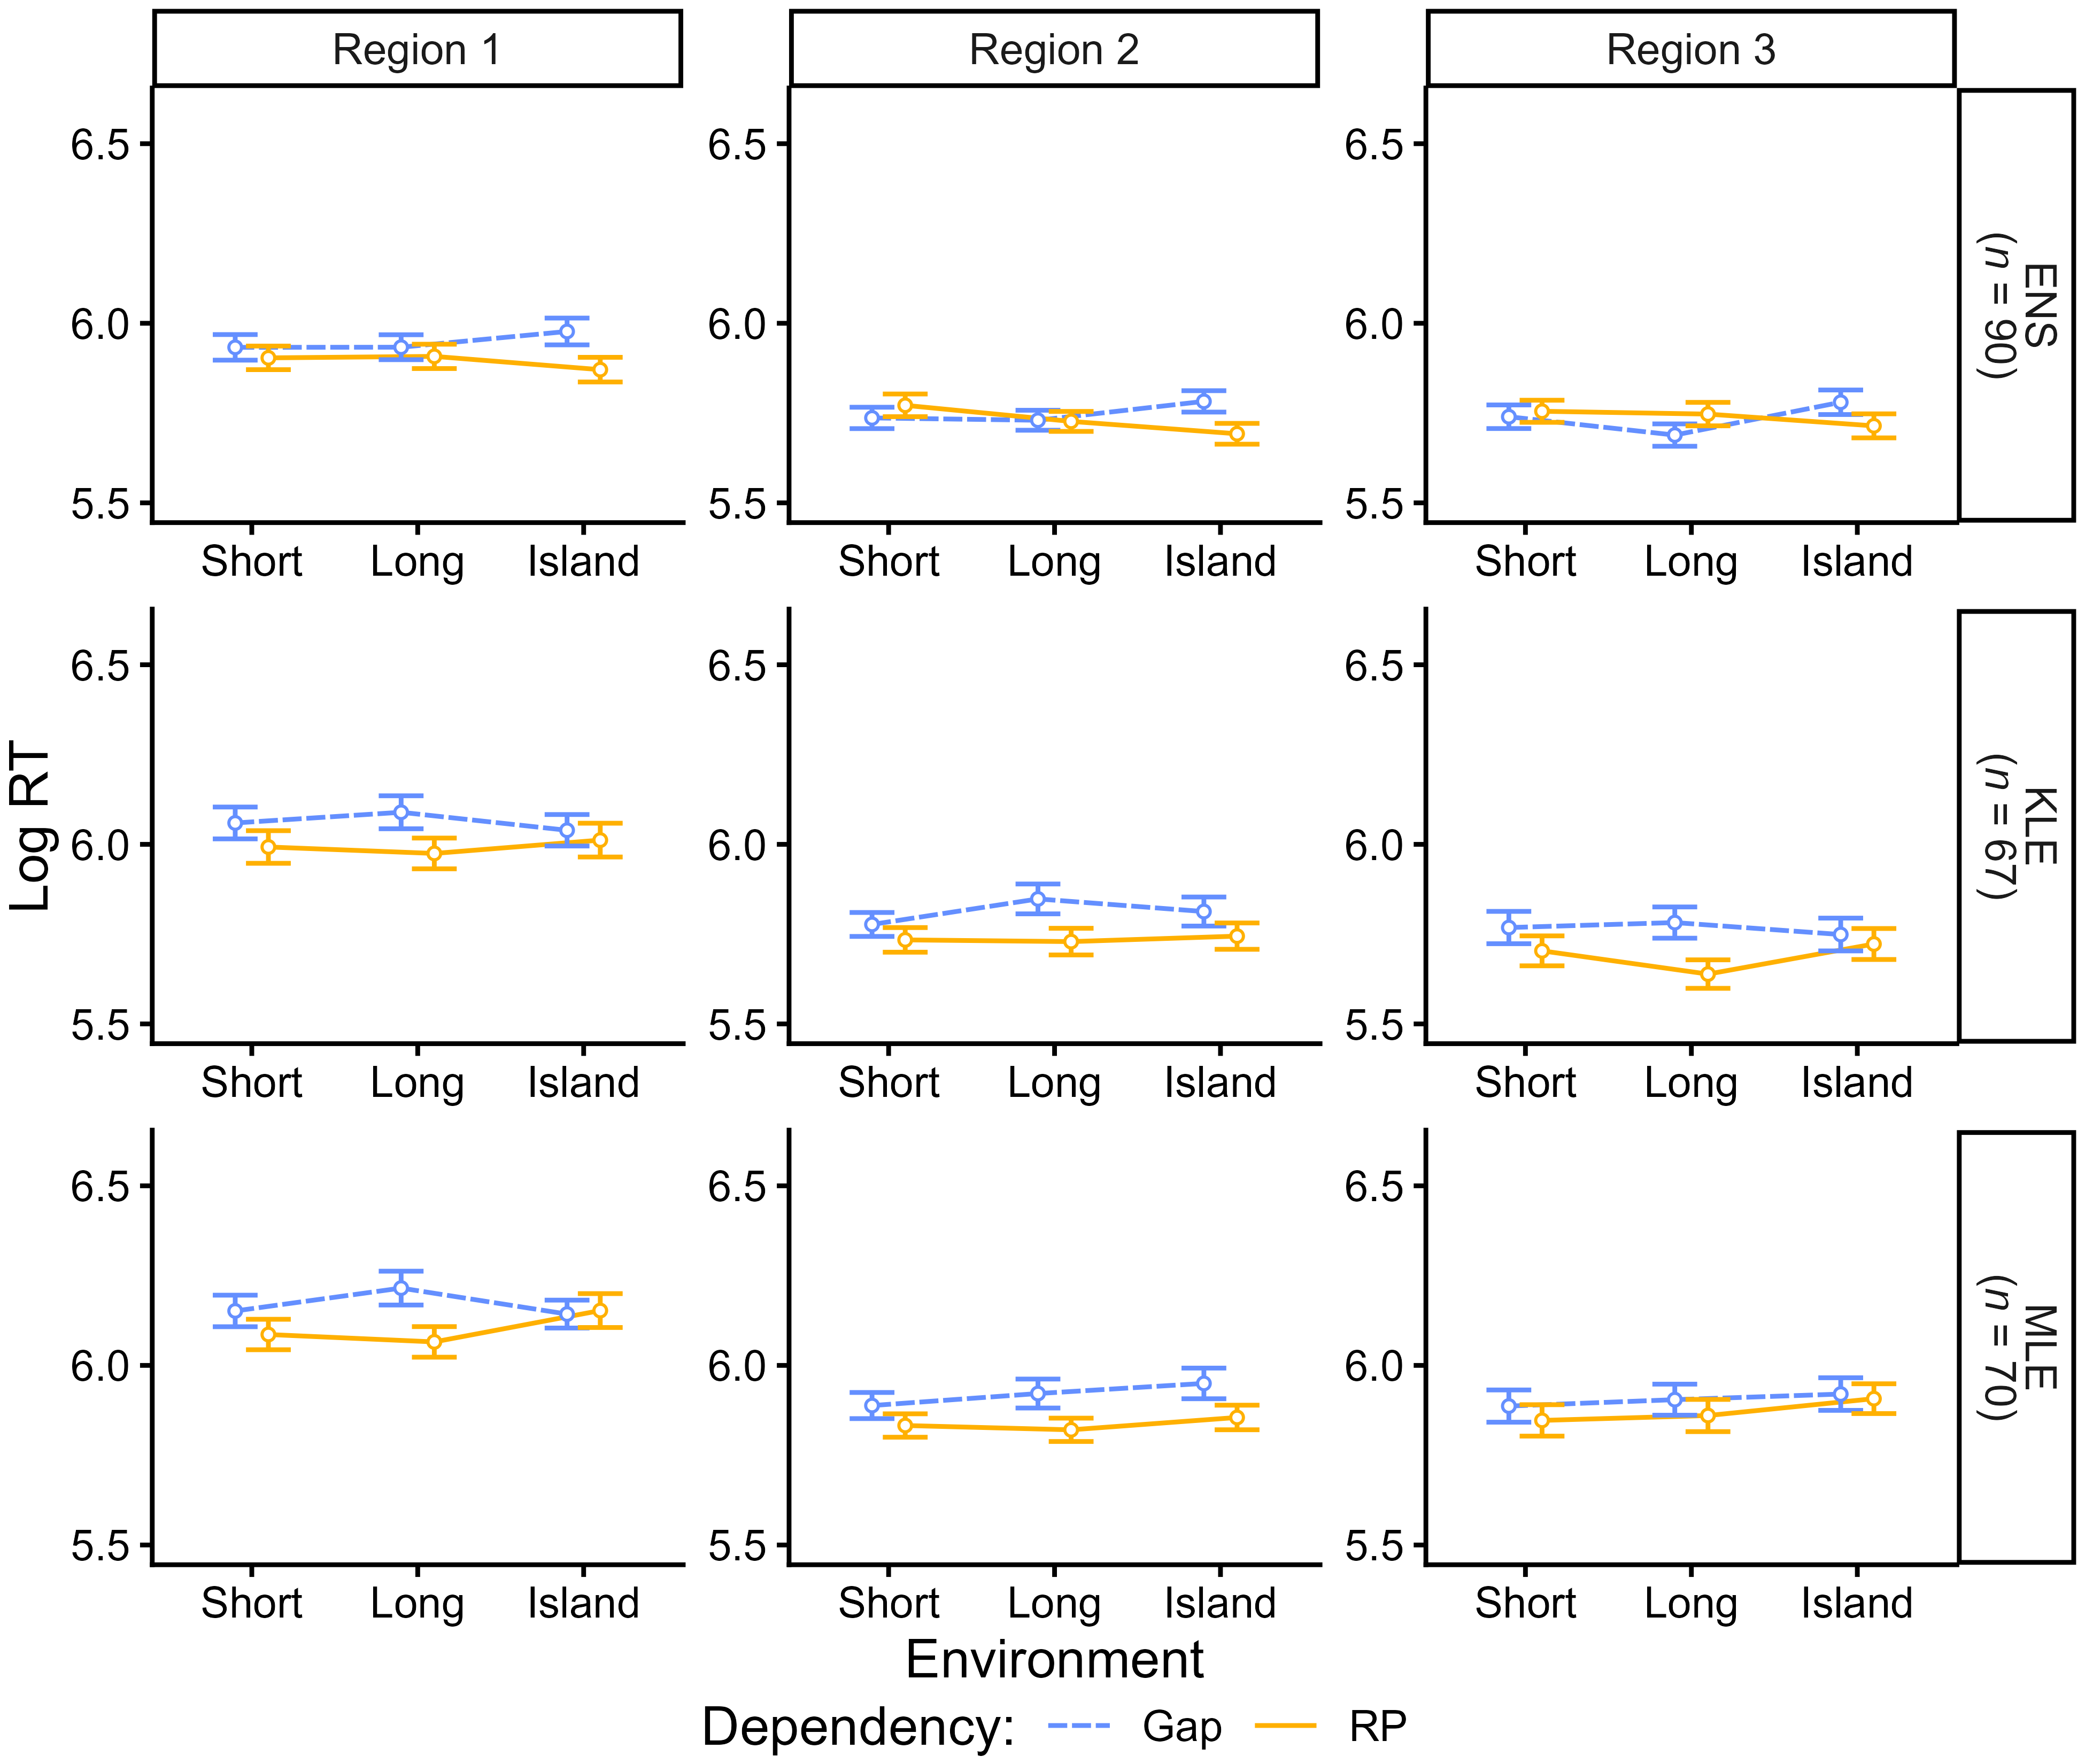
\includegraphics[width=\textwidth]{../analysis/plots/orc_spr_logrt2.png}
\textit{Note}. Error bars are 95\% \textit{CI}s.
\vspace{-12pt}
\end{figure}

\begin{figure}
\caption{Mean log RTs at the regions of interest in the SRC self-paced reading task} \label{fig:spr-logrt-src}
\raggedright\setstretch{1}
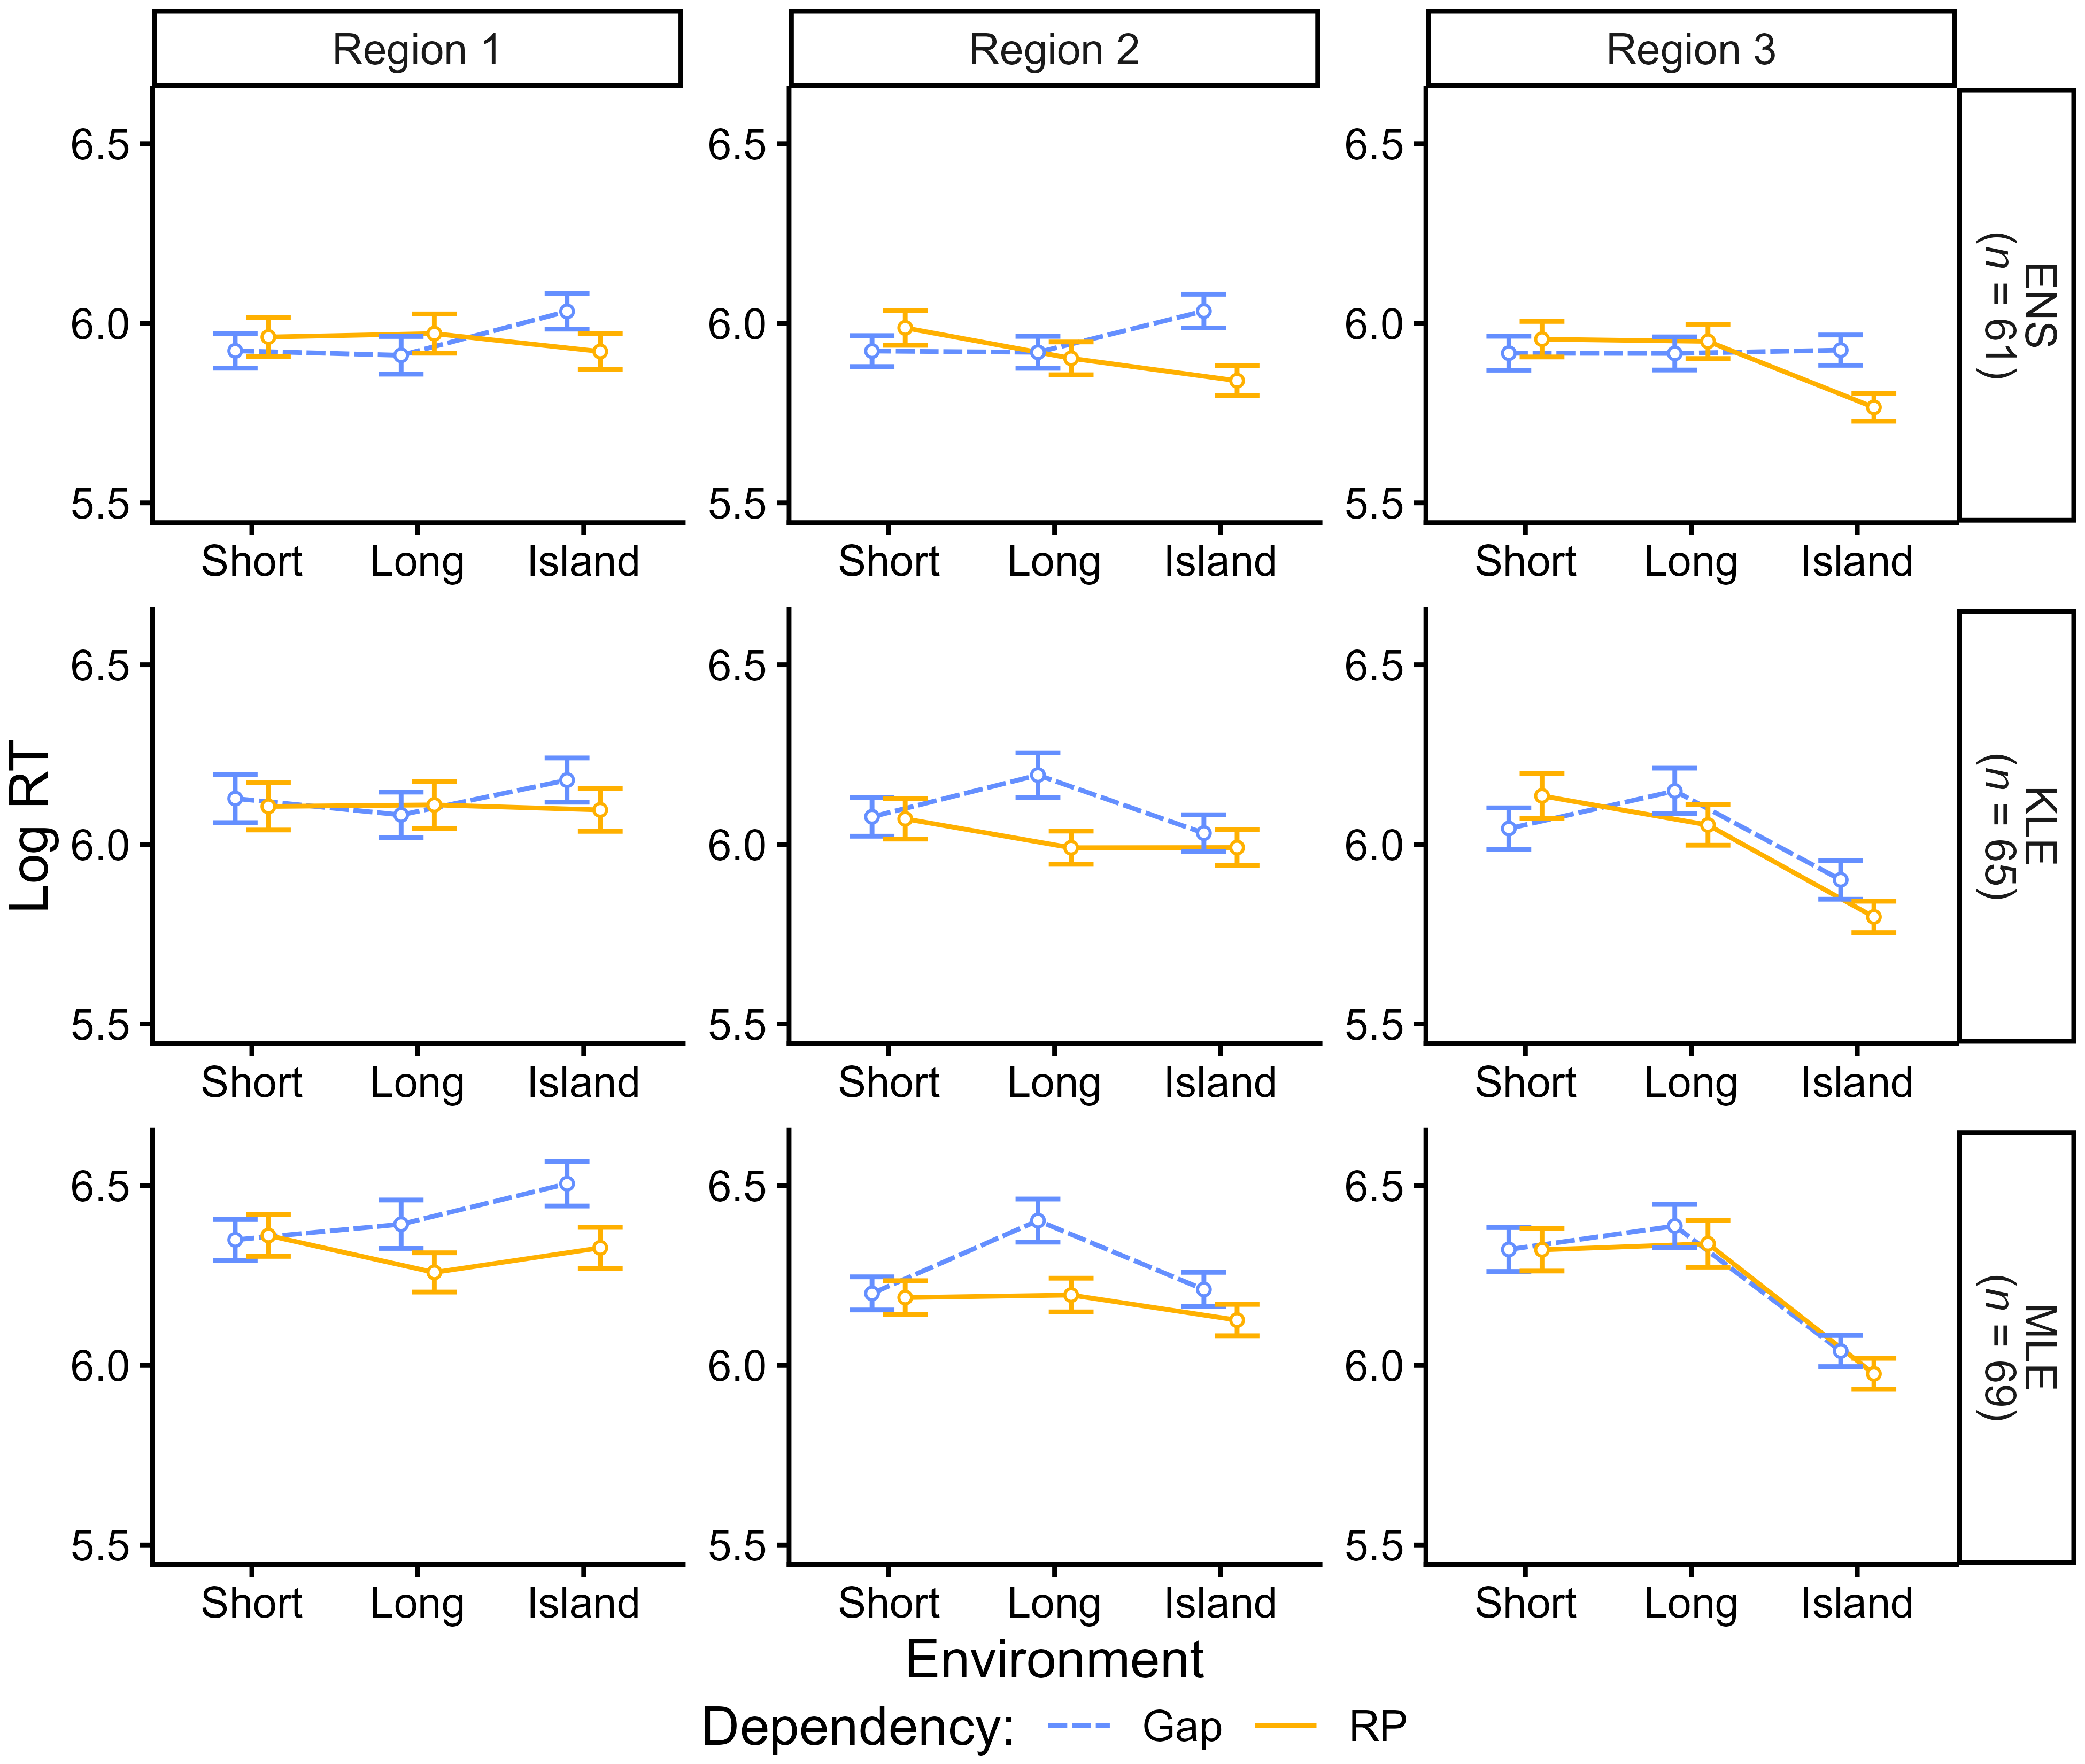
\includegraphics[width=\textwidth]{../analysis/plots/src_spr_logrt2.png}
\textit{Note}. Error bars are 95\% \textit{CI}s.
\vspace{-12pt}
\end{figure}

For ENSs, the relationship between gap-trial RTs and RP-trial RTs varied across environments. In the Short condition, where processing should be easiest, there was a slight numerical advantage for gaps, with gap-trial RTs tending to be faster than RP-trial RTs; this pattern can be seen at Regions 2 and 3 in the ORC dataset and across all three regions in the SRC dataset. In the Island condition, where processing should be hardest, the pattern reversed, and there was a substantial RP advantage in RTs which can be seen across all three regions in both the ORC dataset and the SRC dataset; the non-overlapping error bars suggest that this contrast is likely to be a statistically meaningful one. This pattern of results is consistent with gapping having an edge over resumption in the real-time comprehension of short-distance RCs and resumption having an edge over gapping in the real-time comprehension of \textit{wh}-island RCs.

For L2ers, signs that RPs ease processing relative to gaps can also be seen in several of the environments tested. In the ORC dataset, traces of this RP advantage are visible even in the Short condition, though the contrast is relatively weak there. In many cases, the RP advantage is most pronounced for L2ers in the Long environment. This was certainly the case for KLEs and MLEs across all three regions in the ORC dataset. However, there were also some cases in the SRC dataset where the RP advantage was most pronounced in the Island condition, such as for KLEs at Region~3 and for MLEs at Region~1.

To further examine the patterns in the data, separate linear mixed-effects models were fit to the log RTs for each study and region. 

The ORC Region~1 model (model formula: \textsc{log rt \~{} dependency * environment * group + (1 + dependency + environment | participant) + (1 + dependency + environment + group | item)}---see Appendix~\ref{app-results-spr}, Table~\ref{tab:app-orc-spr-logrt-r1-model} for details) found significant effects for (a)~\textsc{dependency}, with RP trials having faster RTs than gap trials ($\hat{\beta}$~=~−0.06, \textit{SE}~=~0.01, $p$~<~.001), and (b)~\textsc{group}, with KLEs and MLEs both having slower RTs than ENSs (KLE~−~ENS: $\hat{\beta}$~=~0.13, \textit{SE}~=~0.04, $p$~<~.001; MLE~−~ENS: $\hat{\beta}$~=~0.24, \textit{SE}~=~0.04, $p$~<~.001). Two of the three-way \textsc{dependency} × \textsc{environment} × \textsc{group} interactions were significant ($p$~<~.05), showing that the increase in the size of the [RP~−~gap] contrast from the Short condition to the Long condition was larger for KLEs and MLEs than for ENSs. Pairwise comparisons revealed that RP trials were significantly faster than gap trials in the Long condition for KLEs and MLEs (KLE: $\hat{\beta}$~=~−0.09, \textit{SE}~=~0.03, $p$~=~.044; MLE: $\hat{\beta}$~=~−0.12, \textit{SE}~=~0.03, $p$~=~.002) and in the Island condition for ENSs ($\hat{\beta}$~=~−0.11, \textit{SE}~=~0.03, $p$~<~.001). 

The ORC Region~2 model (model formula: \textsc{log rt \~{} dependency * environment * group + (1 + dependency * environment | participant) + (1 + dependency + environment | item)}---see Appendix~\ref{app-results-spr}, Table~\ref{tab:app-orc-spr-logrt-r2-model} for details) yielded (a)~a significant effect for \textsc{dependency}, with RP trials having faster RTs than gap trials ($\hat{\beta}$~=~−0.07, \textit{SE}~=~0.01, $p$~<~.001), (b)~a marginally significant effect for \textsc{environment}, with the Island condition having slower RTs than the Short condition ($\hat{\beta}$~=~0.02, \textit{SE}~=~0.01, $p$~=~.068), and (c)~a significant effect for \textsc{group}, with MLEs having slower RTs than ENSs ($\hat{\beta}$~=~0.15, \textit{SE}~=~0.03, $p$~<~.001). Several of the two-way and three-way interactions reached at least marginal significance. Pairwise comparisons showed that the [RP~−~gap] contrast was marginally significant for MLEs in the Short condition ($\hat{\beta}$~=~−0.07, \textit{SE}~=~0.03, $p$~=~.074), significant for KLEs and MLEs in the Long condition (KLE: $\hat{\beta}$~=~−0.14, \textit{SE}~=~0.03, $p$~<~.001; MLE: $\hat{\beta}$~=~−0.12, \textit{SE}~=~0.03, $p$~<~.001), and significant for all three groups in the Island condition (ENS: $\hat{\beta}$~=~−0.08, \textit{SE}~=~0.03, $p$~=~.016; KLE: $\hat{\beta}$~=~−0.09, \textit{SE}~=~0.03, $p$~=~.015; MLE: $\hat{\beta}$~=~−0.12, \textit{SE}~=~0.03, $p$~<~.001).

The ORC Region~3 model (model formula: \textsc{log rt \~{} dependency * environment * group + (1 + dependency * environment | participant) + (1 + dependency + environment + group | item)}---see Appendix~\ref{app-results-spr}, Table~\ref{tab:app-orc-spr-logrt-r3-model} for details) found significant effects for (a)~\textsc{dependency}, with RP trials having faster RTs than gap trials ($\hat{\beta}$~=~−0.04, \textit{SE}~=~0.01, $p$~=~.002), and (b)~\textsc{group}, with MLEs having slower RTs than ENSs ($\hat{\beta}$~=~0.17, \textit{SE}~=~0.04, $p$~<~.001). Several of the two-way and three-way interactions also reached statistical significance ($p$~<~.05), and pairwise comparisons revealed that the [RP~−~gap] contrast was statistically meaningful only for KLEs, and only in the Long condition ($\hat{\beta}$~=~−0.12, \textit{SE}~=~0.03, $p$~<~.001).

As for the SRC dataset, the SRC Region~1 model (model formula: \textsc{log rt \~{} dependency * environment * group + (1 | participant) + (1 + dependency + environment + group | item)}---see Appendix~\ref{app-results-spr}, Table~\ref{tab:app-src-spr-logrt-r1-model} for details) found significant effects for (a)~\textsc{dependency}, with RP trials having faster RTs than gap trials ($\hat{\beta}$~=~−0.03, \textit{SE}~=~0.01, $p$~=~.014), (b)~\textsc{environment}, with the Island condition having slower RTs than the Short condition ($\hat{\beta}$~=~0.03, \textit{SE}~=~0.02, $p$~=~.049), and (c)~\textsc{group}, with KLEs and MLEs both having slower RTs than ENSs (KLE~−~ENS: $\hat{\beta}$~=~0.19, \textit{SE}~=~0.07, $p$~=~.006; MLE~−~ENS: $\hat{\beta}$~=~0.44, \textit{SE}~=~0.07, $p$~<~.001). Several of the two-way and three-way interactions also came out as significant ($p$~<~.05), and pairwise comparisons found the [RP~−~gap] contrast to be statistically meaningful only for MLEs, and only in the Long and Island conditions (Long: $\hat{\beta}$~=~−0.13, \textit{SE}~=~0.04, $p$~=~.005; Island: $\hat{\beta}$~=~−0.16, \textit{SE}~=~0.04, $p$~<~.001).

The SRC Region~2 model (model formula: \textsc{log rt \~{} dependency * environment * group + (1 + dependency * environment | participant) + (1 + dependency + environment + group | item)}---see Appendix~\ref{app-results-spr}, Table~\ref{tab:app-src-spr-logrt-r2-model} for details) yielded significant effects for (a)~\textsc{dependency}, with RP trials having faster RTs than gap trials ($\hat{\beta}$~=~−0.08, \textit{SE}~=~0.01, $p$~>~.001), (b)~\textsc{environment}, with the Short condition having faster RTs than the Long condition but slower RTs than the Island condition (Long~−~Short: $\hat{\beta}$~=~0.03, \textit{SE}~=~0.02, $p$~=~.028; Island~−~Short: $\hat{\beta}$~=~−0.03, \textit{SE}~=~0.02, $p$~=~.039), and (c)~\textsc{group}, with KLEs and MLEs both having slower RTs than ENSs (KLE~−~ENS: $\hat{\beta}$~=~0.14, \textit{SE}~=~0.05, $p$~=~.011; MLE~−~ENS: $\hat{\beta}$~=~0.30, \textit{SE}~=~0.05, $p$~<~.001). Several of the two-way and three-way interactions were also found to be significant ($p$~<~.05). Follow-up pairwise comparisons revealed that the [RP~−~gap] contrast was significant in the Long condition for KLEs and MLEs (KLE: $\hat{\beta}$~=~−0.19, \textit{SE}~=~0.04, $p$~<~.001; MLE: $\hat{\beta}$~=~−0.21, \textit{SE}~=~0.04, $p$~<~.001) and in the Island condition for ENSs and MLEs (ENS: $\hat{\beta}$~=~−0.20, \textit{SE}~=~0.03, $p$~<~.001; MLE: $\hat{\beta}$~=~−0.10, \textit{SE}~=~0.03, $p$~=~.028).

Finally, the SRC Region~3 model (model formula: \textsc{log rt \~{} dependency * environment * group + (1 + dependency * environment | participant) + (1 + dependency + environment + group | item)}---see Appendix~\ref{app-results-spr}, Table~\ref{tab:app-src-spr-logrt-r3-model} for details) found (a)~a significant effect for \textsc{dependency}, with RP trials having faster RTs than gap trials ($\hat{\beta}$~=~−0.04, \textit{SE}~=~0.01, $p$~=~.007), (b)~a marginally significant effect for \textsc{environment}, with Island trials having faster RTs than Short trials ($\hat{\beta}$~=~−0.24, \textit{SE}~=~0.03, $p$~<~.001), and (c)~a significant effect for \textsc{group}, with KLEs and MLEs both having slower RTs than ENSs (KLE~−~ENS: $\hat{\beta}$~=~0.12, \textit{SE}~=~0.06, $p$~=~.049; MLE~−~ENS: $\hat{\beta}$~=~0.35, \textit{SE}~=~0.06, $p$~<~.001). Several of the two-way and three-way interactions also came out as significant, and pairwise comparisons showed that the [RP~−~gap] contrast was marginally significant for KLEs in the Short condition, with RP trials having slower RTs than gap trials ($\hat{\beta}$~=~0.11, \textit{SE}~=~0.04, $p$~=~.057), and significant for both ENSs and KLEs in the Island condition, with RP trials having faster RTs than gap trials (ENS: $\hat{\beta}$~=~−0.14, \textit{SE}~=~0.04, $p$~<~.001; KLE: $\hat{\beta}$~=~−0.13, \textit{SE}~=~0.03, $p$~=~.001).

To review, all groups had faster RTs with RPs than with gaps in the Island condition, where processing should be hardest, for at least one of the three regions of interest. The L2ers also displayed an RP advantage in Long-condition RTs for one or more regions in both the ORC dataset and the SRC dataset. None of the groups displayed a significant RP advantage in the Short environment, where processing should be easiest. In fact, ENSs almost invariably exhibited a slight numerical advantage for gaps in the Short condition, suggesting that RCs may actually hinder processing in environments where the dependency is very easy to resolve with a gap. KLEs similarly displayed a marginally significant gap advantage in the Short condition, but only at Region~3, and only in the SRC dataset. Overall, this pattern of results is consistent with RPs facilitating real-time comprehension of RCs when there is strain on the processor. However, faster RTs are not always indicative of processing facilitation; sometimes, they simply indicate that the participant has abandoned the parse (\cite{morgan.etal2020}, p.~3; \cite{nicenboim.etal2016}, p.~11). In Section~\ref{spr-accuracy}, we will inspect participants' accuracy rates in the comprehension questions to check their consistency in correctly resolving the RC dependency in RP trials.

%========================================================%
\section{L2 proficiency effects for RTs at the regions of interest}\label{spr-rt-proficiency}
%========================================================%

Let us now examine how L2 proficiency related to RTs at the regions of interest. For this analysis, I focus on Region~1 RTs for the ORC dataset and Region~2 RTs for the SRC dataset. I selected those regions because (a)~they were the first regions where all groups exhibited a significant [RP~−~gap] contrast and (b)~they were the regions with the greatest [RP~−~gap] difference score, averaged across all levels of \textsc{environment} and \textsc{group} (see Appendix~\ref{app-results-spr}, Table~\ref{tab:app-spr-dscore} for details). There was one MLE in the SRC dataset who could not be included in this analysis due to a missing proficiency score.

Figures \ref{fig:spr-rt-proficiency-orc} and \ref{fig:spr-rt-proficiency-src} show the relationship between L2ers' scaled English proficiency scores and their mean log RTs in, respectively, the ORC data and the SRC data.\footnotemark{}

\footnotetext{See Section~\ref{stu-analysis} for the logic behind scaling the proficiency scores prior to modeling; scaling was done separately for the ORC data and the SRC data.}

\begin{figure}
\caption{Relationship between L2 proficiency and Region~1 log RTs in the ORC self-paced reading task} \label{fig:spr-rt-proficiency-orc}
\raggedright\setstretch{1}
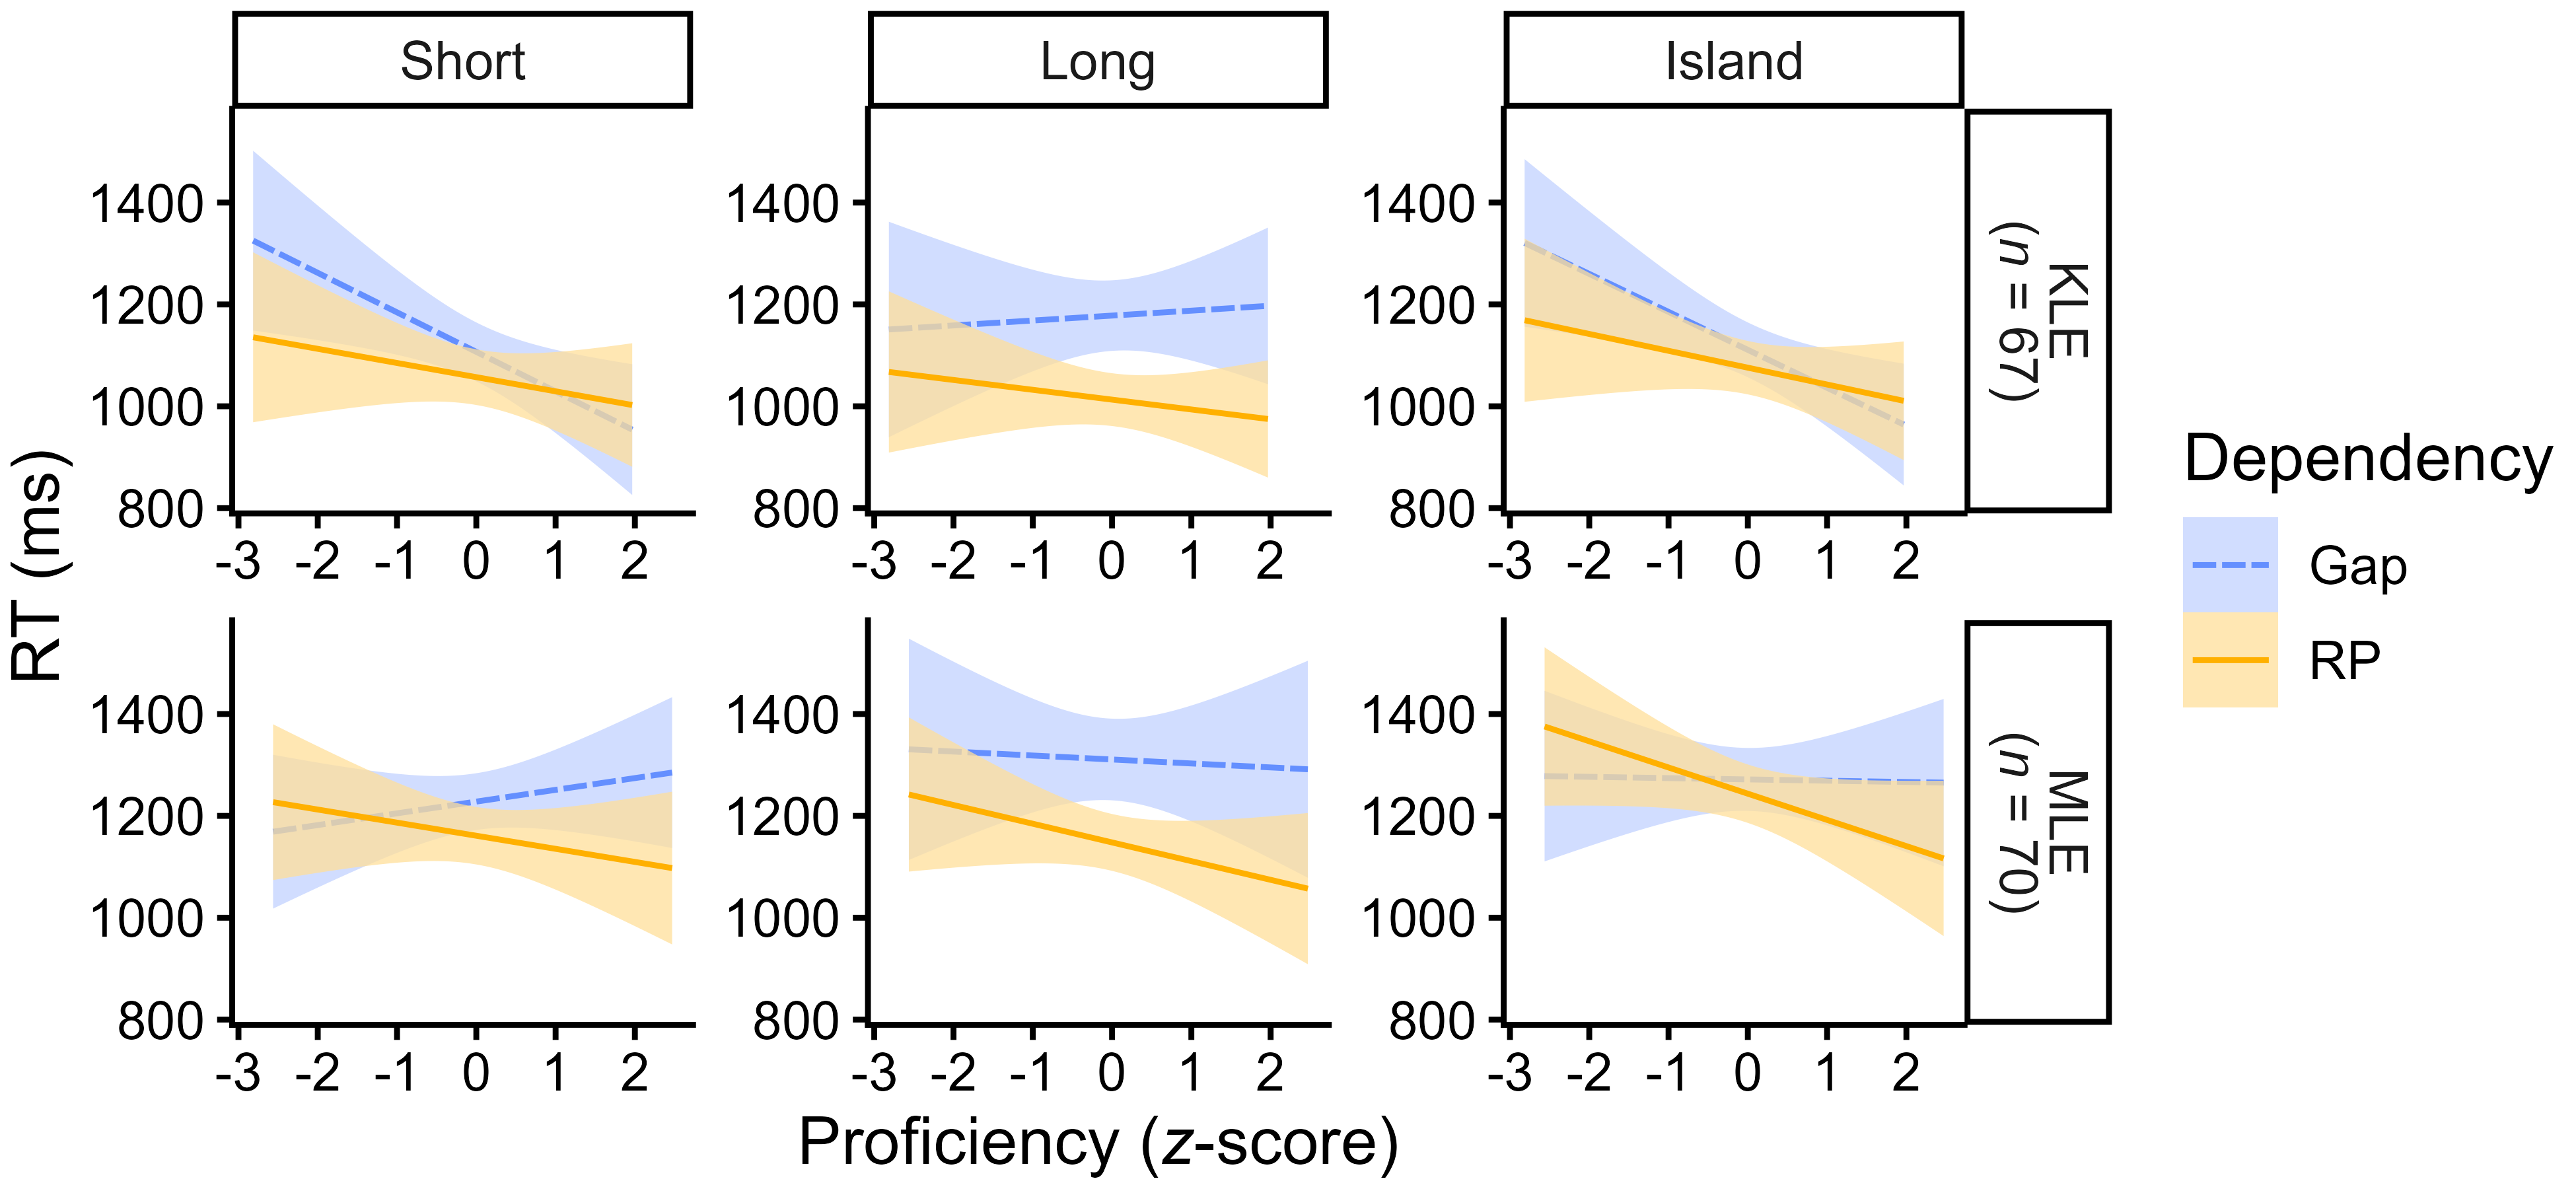
\includegraphics[width=\textwidth]{../analysis/plots/orc_spr_rt_proficiency.png}
\textit{Note}. Shading indicates 95\% \textit{CI}s.
\vspace{-12pt}
\end{figure}

\begin{figure}
\caption{Relationship between L2 proficiency and Region~2 log RTs in the SRC self-paced reading task} \label{fig:spr-rt-proficiency-src}
\raggedright\setstretch{1}
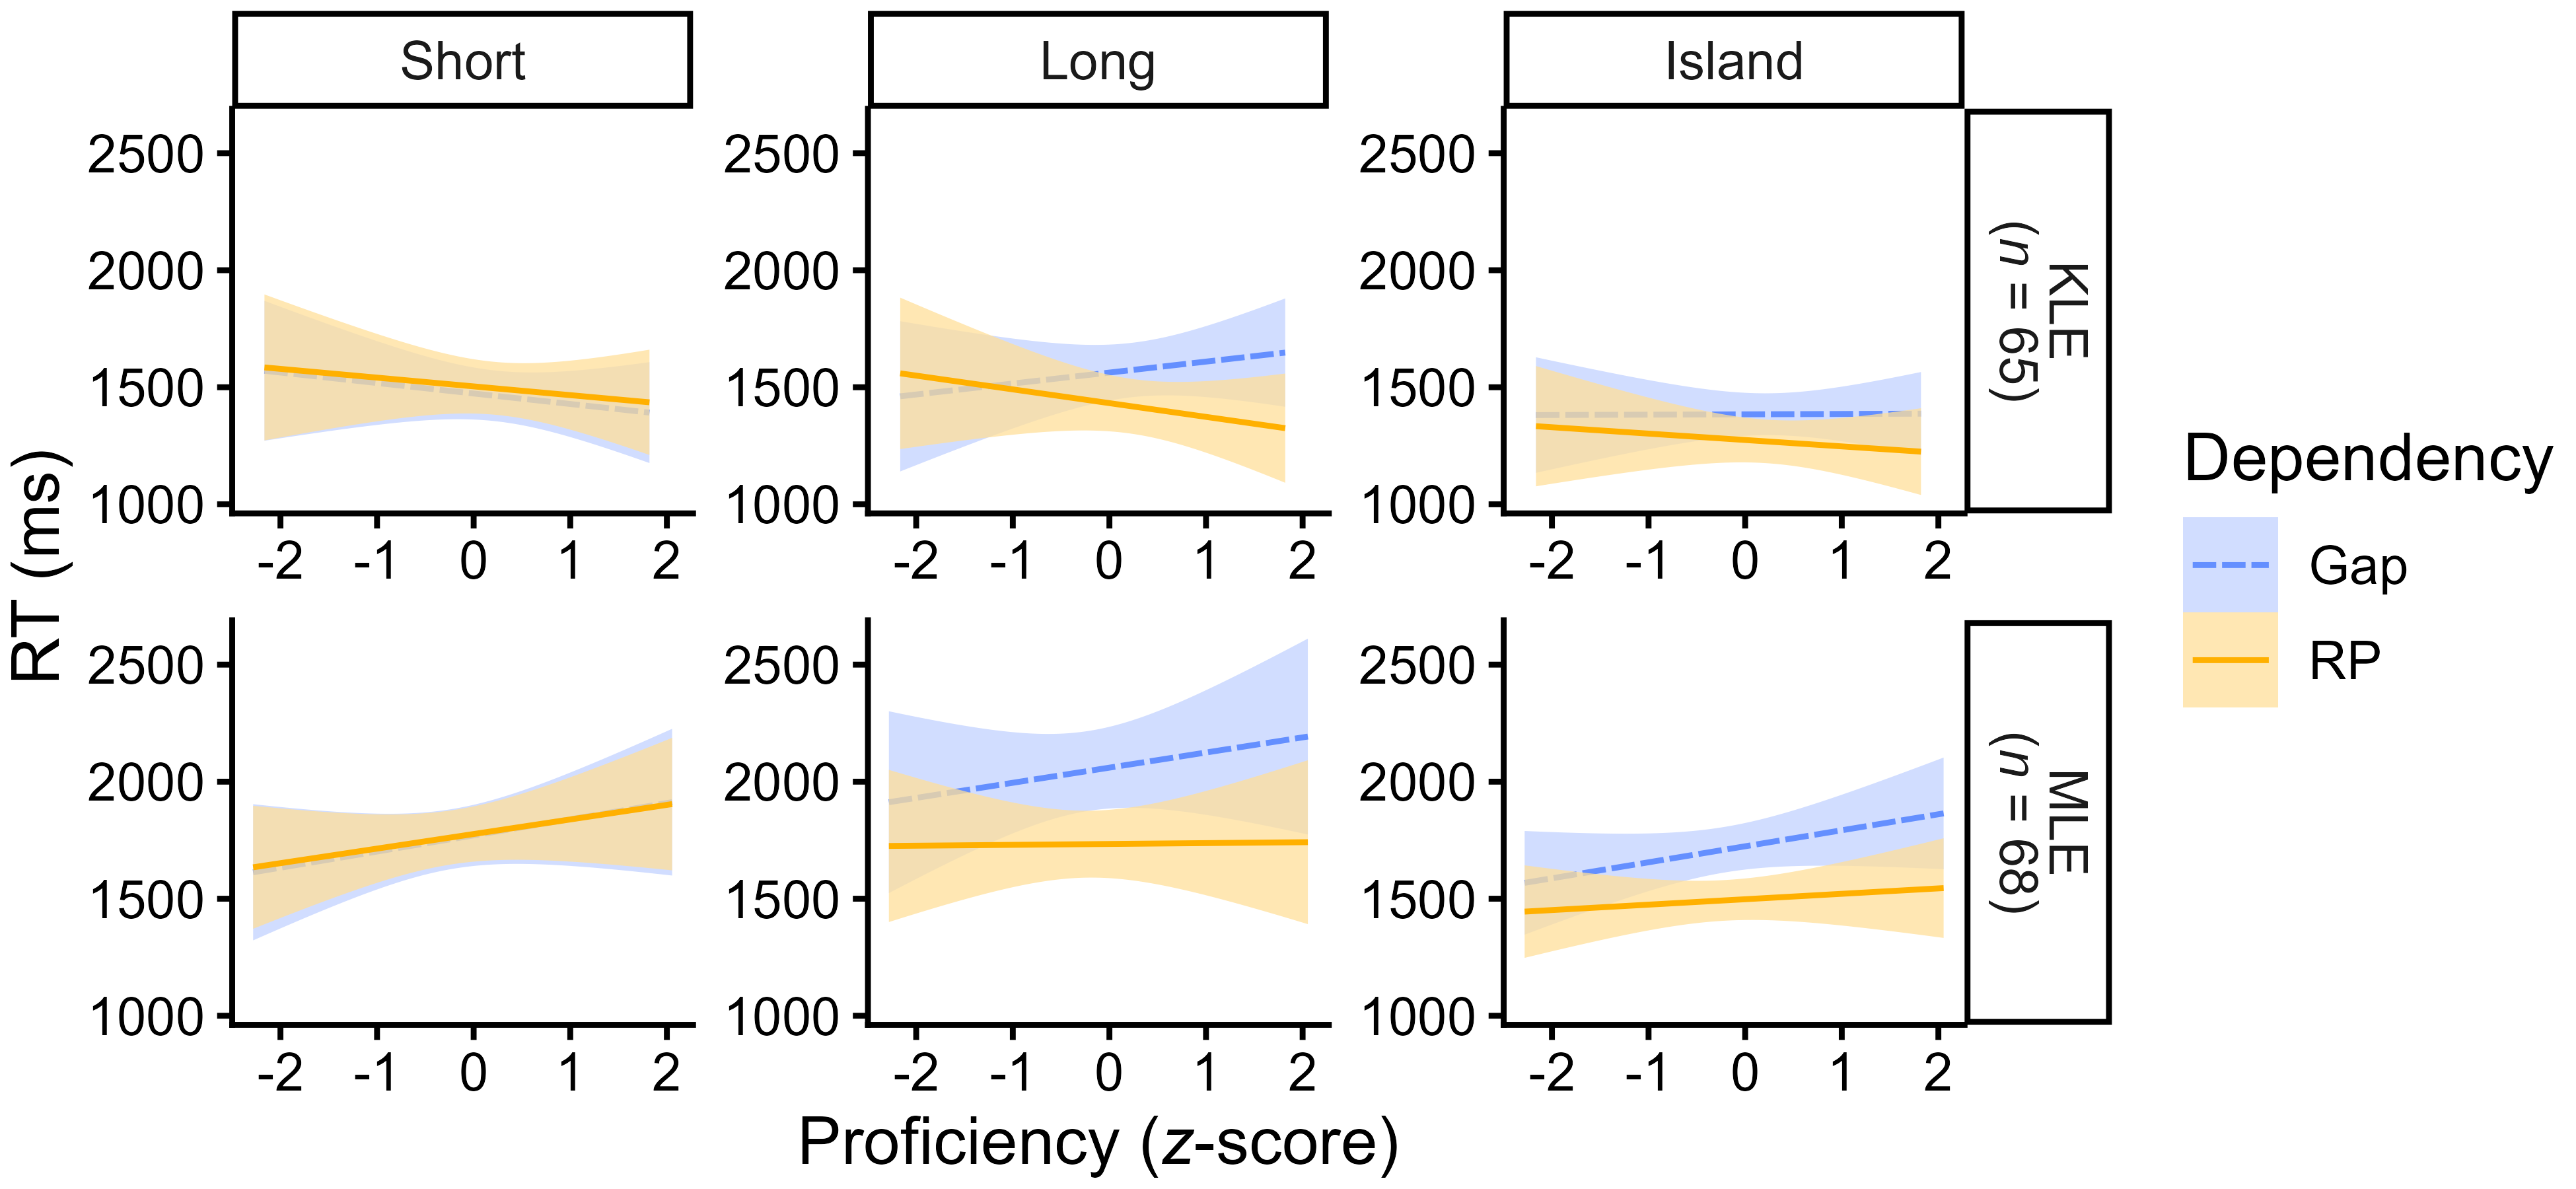
\includegraphics[width=\textwidth]{../analysis/plots/src_spr_rt_proficiency.png}
\textit{Note}. Shading indicates 95\% \textit{CI}s.
\vspace{-12pt}
\end{figure}

\noindent Although we can see that there was a clear RP advantage in RTs in the Long condition and also, albeit on a more modest scale, in the Short and Island conditions, no strong \textsc{dependency × proficiency} interaction is visible for any combination of \textsc{environment} and \textsc{group}. If such an interaction were present, the trend lines for gaps and RPs in the plots would have radically different slopes, forming an `X' shape or a sideways `V' shape.

To further probe for L2 proficiency effects in the RT data, I refit the linear mixed-effects models for the ORC data and the SRC data separately with \textsc{proficiency} added as a continuous fixed effect. 

The ORC model (model formula: \textsc{log rt \~{} dependency * environment * group * proficiency + (1 + dependency * environment | participant) + (1 + dependency + environment + group | item)}---see Appendix~\ref{app-results-spr}, Table \ref{tab:app-orc-spr-logrt-proficiency-model} for details) found a significant negative relationship between L2 proficiency scores and RTs ($\hat{\beta}$~=~−0.04, \textit{SE}~=~0.02, $p$~=~.015). That is to say, as proficiency increased, RTs across conditions tended to get somewhat faster. However, the \textsc{dependency} × \textsc{proficiency} interaction did not reach significance ($\hat{\beta}$~=~−0.01, \textit{SE}~=~0.01, $p$~=~.378), signaling the absence of a meaningful relationship between proficiency scores and the strength of the RP advantage in RTs (cf.~the L2 plots in Figures~\ref{fig:spr-logrt-orc} and \ref{fig:spr-logrt-src}). While two of the three-way interactions involving \textsc{proficiency} came out as significant ($p$~<~.05), post-hoc testing did not find the effect of \textsc{proficiency} on the [RP~−~gap] contrast to approach significance in any \textsc{environment} × \textsc{group} combinations (all $p$s~>~.10).

The SRC model (model formula: \textsc{log rt \~{} dependency * environment * group * proficiency + (1 + dependency + environment | participant) + (1 + dependency + environment + group | item)}---see Appendix~\ref{app-results-spr}, Table~\ref{tab:app-src-spr-logrt-proficiency-model} for details) did not find a statistically meaningful effect for \textsc{proficiency} ($\hat{\beta}$~=~0.03, \textit{SE}~=~0.02, $p$~=~.194). The \textsc{dependency × proficiency} interaction did not reach significance, either ($\hat{\beta}$~=~−0.01, \textit{SE}~=~0.01, $p$~=~.494). Although several of the three-way interactions involving \textsc{proficiency} did reach significance, post-hoc tests did not find the proficiency trend for the [RP~−~gap] contrast to approach significance for any combinations of \textsc{environment} and \textsc{group} (all $p$s~>~.10). 

This analysis, in short, did not find evidence that the strength of the RT advantage for RPs relative to gaps was modulated by L2 proficiency in either the ORC study or the SRC study.

%========================================================%
\section{Comprehension-question accuracy}\label{spr-accuracy}
%========================================================%

Next, let us turn our attention to RQ2, which asks how resumption affects accuracy on comprehension questions. Figures~\ref{fig:spr-accuracy-orc} and \ref{fig:spr-accuracy-src} show the mean rates of comprehension-question accuracy for, respectively, the ORC dataset and the SRC dataset. Strikingly, the mean accuracy scores were consistently higher in RP trials than in gap trials across all levels of \textsc{environment} and \textsc{group}. Whereas the magnitude of the RP advantage was more or less steady across conditions in the ORC data, it increased across conditions in the SRC data, with the size of the difference being larger in the Long and Island conditions than in the Short condition.

\begin{figure}
\caption{Mean accuracy on comprehension questions in the ORC self-paced reading task} \label{fig:spr-accuracy-orc}
\raggedright\setstretch{1}
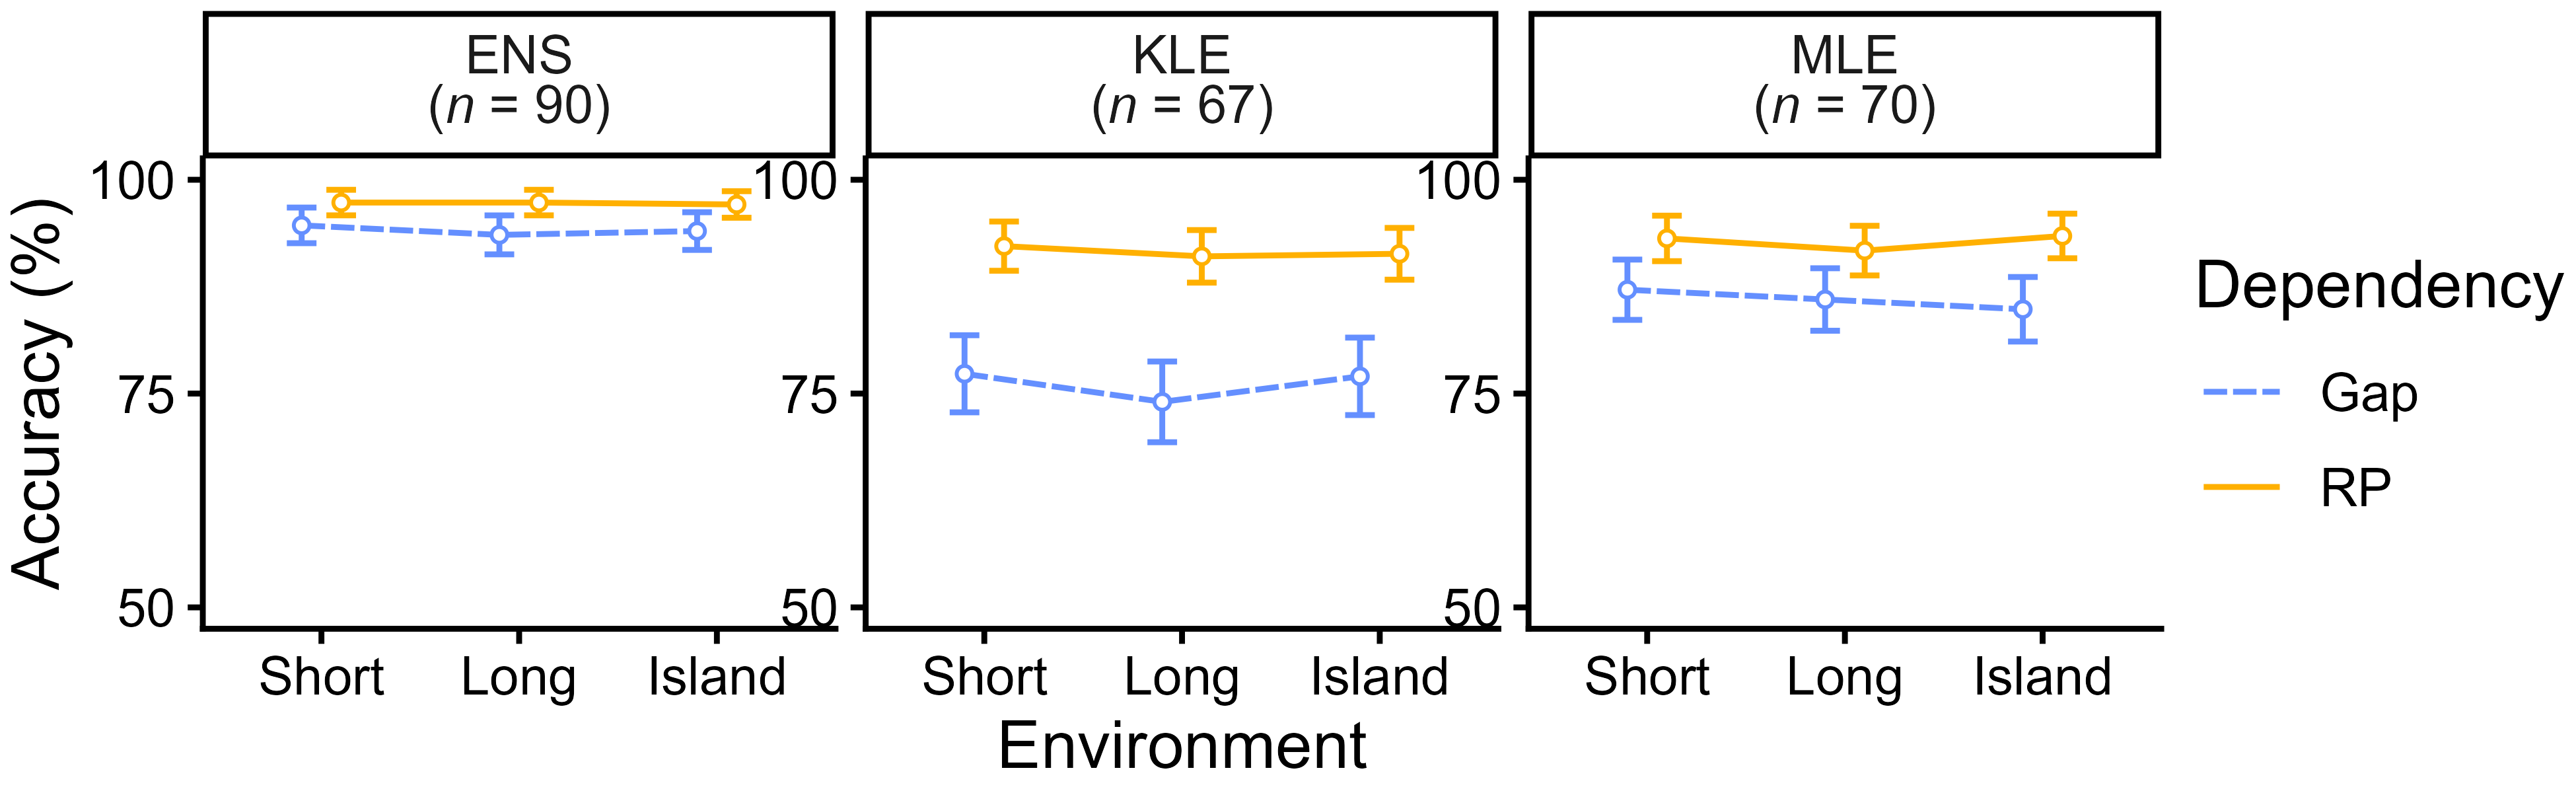
\includegraphics[width=\textwidth]{../analysis/plots/orc_spr_accuracy.png}
\textit{Note}. Error bars are 95\% \textit{CI}s.
\vspace{-12pt}
\end{figure}

\begin{figure}
\caption{Mean accuracy on comprehension questions in the SRC self-paced reading task} \label{fig:spr-accuracy-src}
\raggedright\setstretch{1}
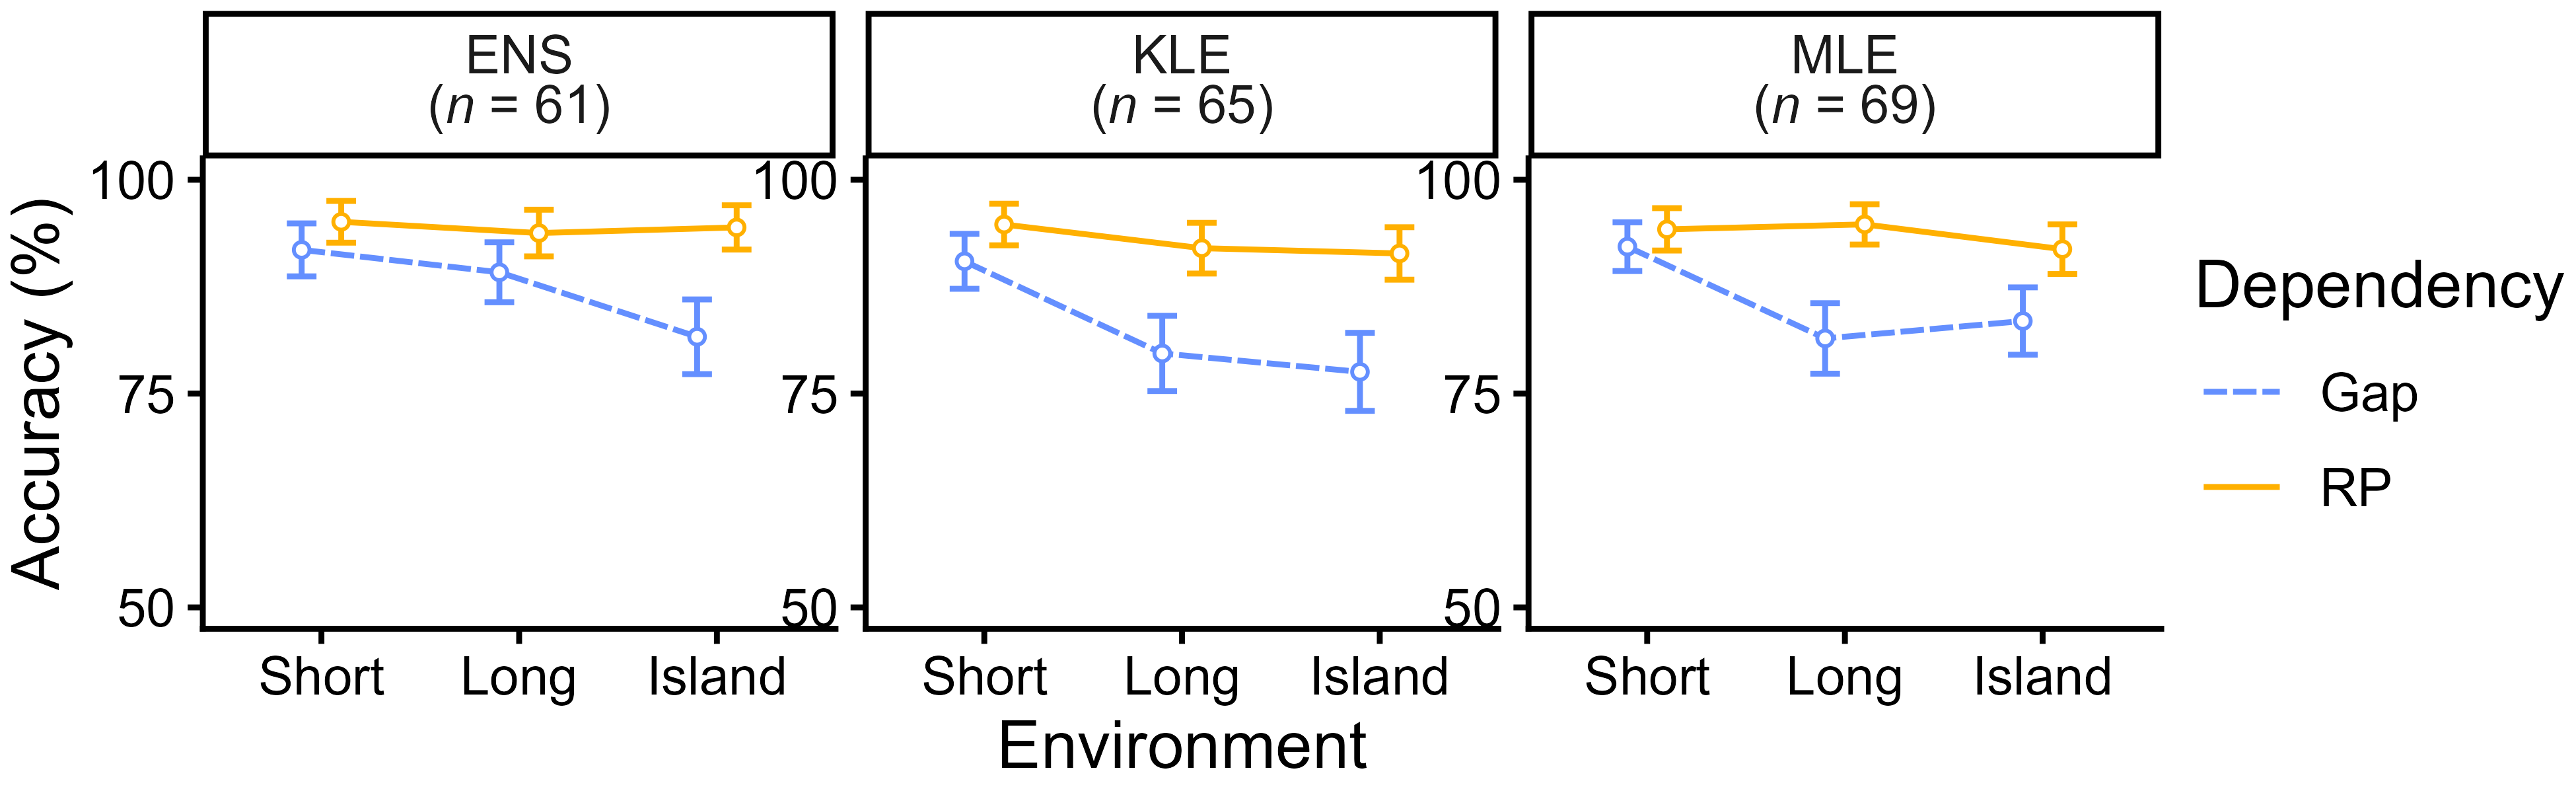
\includegraphics[width=\textwidth]{../analysis/plots/src_spr_accuracy.png}
\textit{Note}. Error bars are 95\% \textit{CI}s.
\vspace{-12pt}
\end{figure}

Performance on filler trials (see Appendix~\ref{app-results-spr}, Figures~\ref{fig:app-orc-spr-accuracy-filler} and \ref{fig:app-src-spr-accuracy-filler}) was checked to confirm that comprehension-question accuracy was high for at least grammatical items (the expected result if the task is functioning as it should). Accuracy was indeed high when averaged across grammatical fillers (above 80\% for all {\sc group} × {\sc study} combinations) and somewhat lower when averaged across ungrammatical fillers, as shown in Table~\ref{tab:spr-fill}.

\begin{table}
\caption{Filler accuracy in the ORC and SRC self-paced reading tasks}\label{tab:spr-fill}
\raggedright\setstretch{1}
\begin{tblr}{colspec={llrrr}}\toprule
Study~~ & Grammaticality~~ & ENS Accuracy (\%) & ~~KLE Accuracy (\%) & ~~MLE Accuracy (\%) \\\midrule
ORC & Grammatical & 86.90 & 84.97 & 84.95 \\
SRC & Grammatical & 86.89 & 82.75 & 84.37 \\
ORC & Ungrammatical & 82.28 & 76.77 & 77.53 \\
SRC & Ungrammatical & 84.40 & 74.33 & 75.07 \\
\bottomrule
\end{tblr}
\vspace{-12pt}
\end{table}

I examined the critical-trial data in more detail by fitting the binary accuracy scores from the ORC and SRC datasets to separate logistic mixed-effects regression models. 

The ORC model (model formula: \textsc{accuracy \~{} dependency * environment * group + (1 + dependency + environment | participant) + (1 + dependency + environment + group | item)}---see Appendix~\ref{app-results-spr}, Table~\ref{tab:app-orc-spr-accuracy-model} for details) showed that overall accuracy was significantly higher for RPs than for gaps ($\hat{\beta}$~=~1.01, \textit{SE}~=~0.17, $p$~<~.001). Accuracy was also significantly higher for ENSs than for KLEs ($\hat{\beta}$~=~−1.72, \textit{SE}~=~0.27, $p$~<~.001) and MLEs ($\hat{\beta}$~=~−0.93, \textit{SE}~=~0.27, $p$~=~.001). The two-way \textsc{dependency}[RP~−~gap] × \textsc{group}[KLE~−~ENS] interaction came out as significant as well ($\hat{\beta}$~=~0.65, \textit{SE}~=~0.28, $p$~=~.018), indicating that the [RP~−~gap] contrast was greater for KLEs than for ENSs. Pairwise comparisons revealed that for ENSs, the contrast did not reach statistical significance in any of the environments tested (all $p$s~>~.05); this may have been due to a ceiling effect, as the ENSs' mean accuracy in each condition was above 95\%. For KLEs, the RP advantage was significant across all three environments (Short: $\hat{\beta}$~=~1.49, \textit{SE}~=~0.30, $p$~<~.001; Long: $\hat{\beta}$~=~1.47, \textit{SE}~=~0.28, $p$~<~.001; Island: $\hat{\beta}$~=~1.35, \textit{SE}~=~0.29, $p$~<~.001). As for MLEs, the RP advantage was significant only in the Island environment ($\hat{\beta}$~=~1.06, \textit{SE}~=~0.34, $p$~=~.015).

The SRC model (model formula: \textsc{accuracy \~{} dependency * environment * group + (1 + dependency + environment | participant) + (1 + dependency + environment + group | item)}---see Appendix~\ref{app-results-spr}, Table~\ref{tab:app-src-spr-accuracy-model} for details) yielded significant effects for (a)~\textsc{dependency}, with RP trials having higher accuracy scores than gap trials ($\hat{\beta}$~=~1.13, \textit{SE}~=~0.17, $p$~<~.001), and (b)~\textsc{environment}, with the Long and Island conditions both having lower accuracy scores than the Short condition (Long~−~Short: $\hat{\beta}$~=~−0.64, \textit{SE}~=~0.23, $p$~=~.006; Island~−~Short: $\hat{\beta}$~=~−0.92, \textit{SE}~=~0.21, $p$~<~.001). One of the two-way \textsc{dependency × environment} interactions and one of the three-way \textsc{dependency × environment × group} interactions also reached marginal significance (.10~>~$p$~>~.05). Pairwise comparisons revealed that the [RP~−~gap] contrast was significant for ENSs in the Island condition ($\hat{\beta}$~=~1.61, \textit{SE}~=~0.34, $p$~<~.001) and for L2ers in both the Long condition (KLE: $\hat{\beta}$~=~1.25, \textit{SE}~=~0.31, $p$~<~.001; MLE: $\hat{\beta}$~=~1.70, \textit{SE}~=~0.34, $p$~<~.001) and the Island condition (KLE: $\hat{\beta}$~=~1.43, \textit{SE}~=~0.30, $p$~<~.001; MLE: $\hat{\beta}$~=~1.01, \textit{SE}~=~0.30, $p$~=~.006). 

These results are indicative of a general RP-over-gap advantage in RC comprehension. For MLEs in the ORC dataset and for all groups in the SRC dataset, this RP advantage grew in strength down the SLW hierarchy (from the Short condition to the Long condition and/or the Island condition), suggesting that it is modulated by processing load. Furthermore, the fact that the RP advantage was larger in the SRC Island condition than in the ORC Island condition, at least for ENSs, is consistent with the idea that in English, \textit{wh}-island SRCs are stronger islands than \textit{wh}-island ORCs.

%========================================================%
\section{L2 proficiency effects for comprehension-question accuracy}\label{spr-accuracy-proficiency}
%========================================================%

Now let us examine how L2 proficiency related to comprehension-question accuracy. The relationship between L2ers' mean accuracy rates and their scaled English proficiency scores is shown in Figures \ref{fig:spr-accuracy-proficiency-orc} and \ref{fig:spr-accuracy-proficiency-src} for, respectively, the ORC data and the SRC data. One MLE in the SRC dataset had to be omitted from this analysis because of a missing proficiency score.

\begin{figure}
\caption{Relationship between L2 proficiency and comprehension-question accuracy in the ORC self-paced reading task} \label{fig:spr-accuracy-proficiency-orc}
\raggedright\setstretch{1}
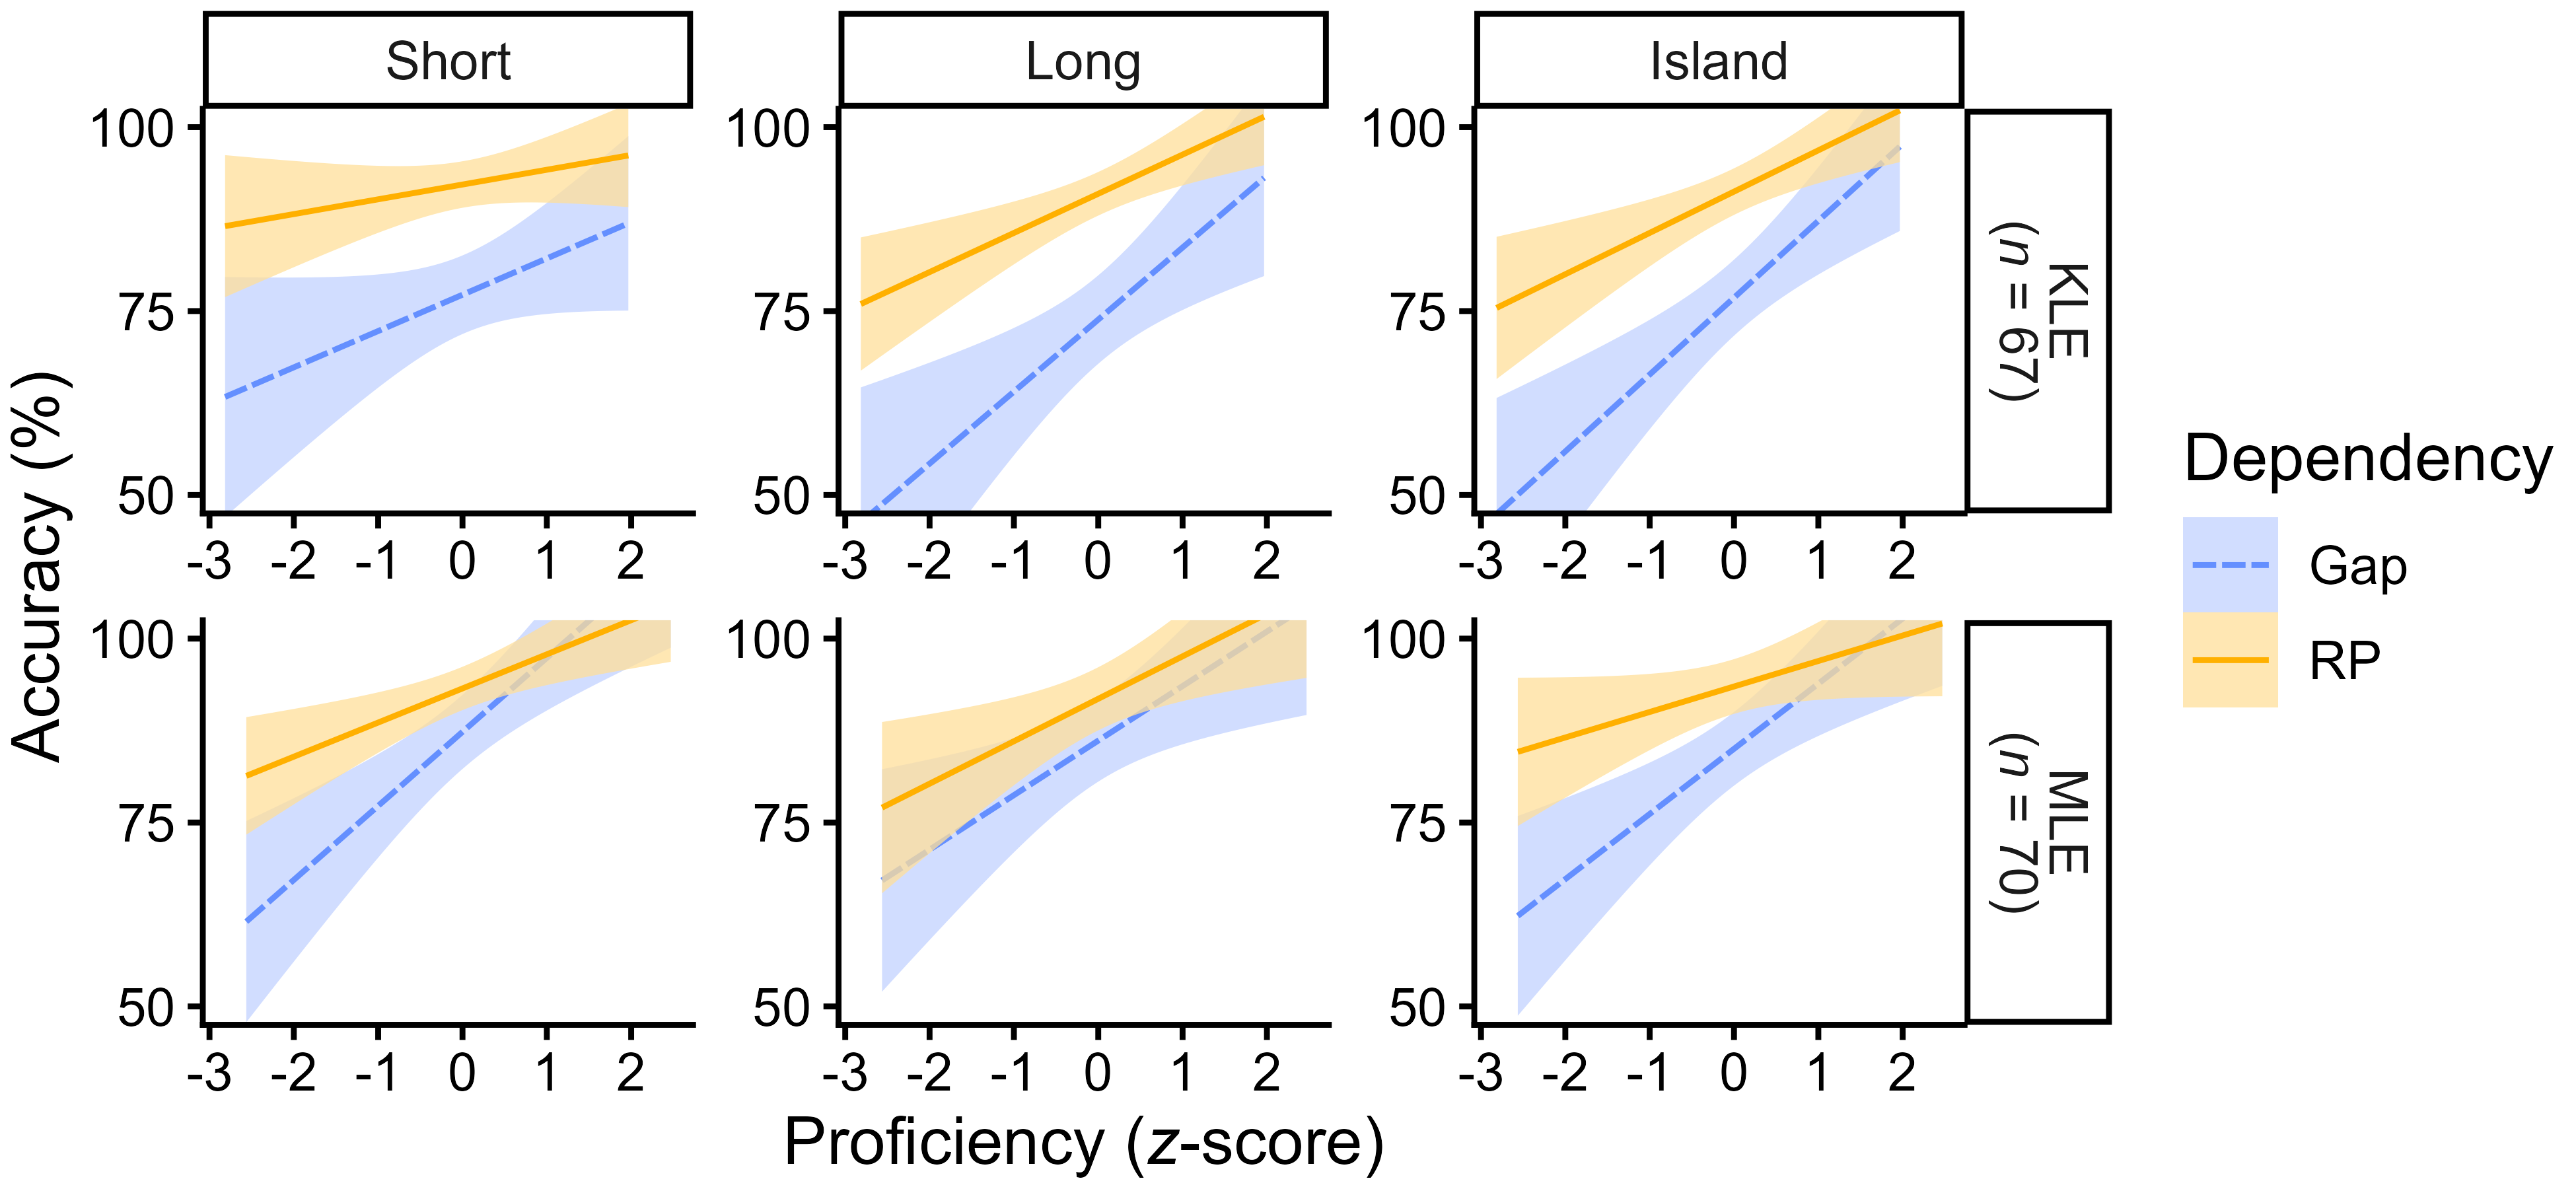
\includegraphics[width=\textwidth]{../analysis/plots/orc_spr_accuracy_proficiency.png}
\textit{Note}. Shading indicates 95\% \textit{CI}s.
\vspace{-12pt}
\end{figure}

\begin{figure}
\caption{Relationship between L2 proficiency and comprehension-question accuracy in the SRC self-paced reading task} \label{fig:spr-accuracy-proficiency-src}
\raggedright\setstretch{1}
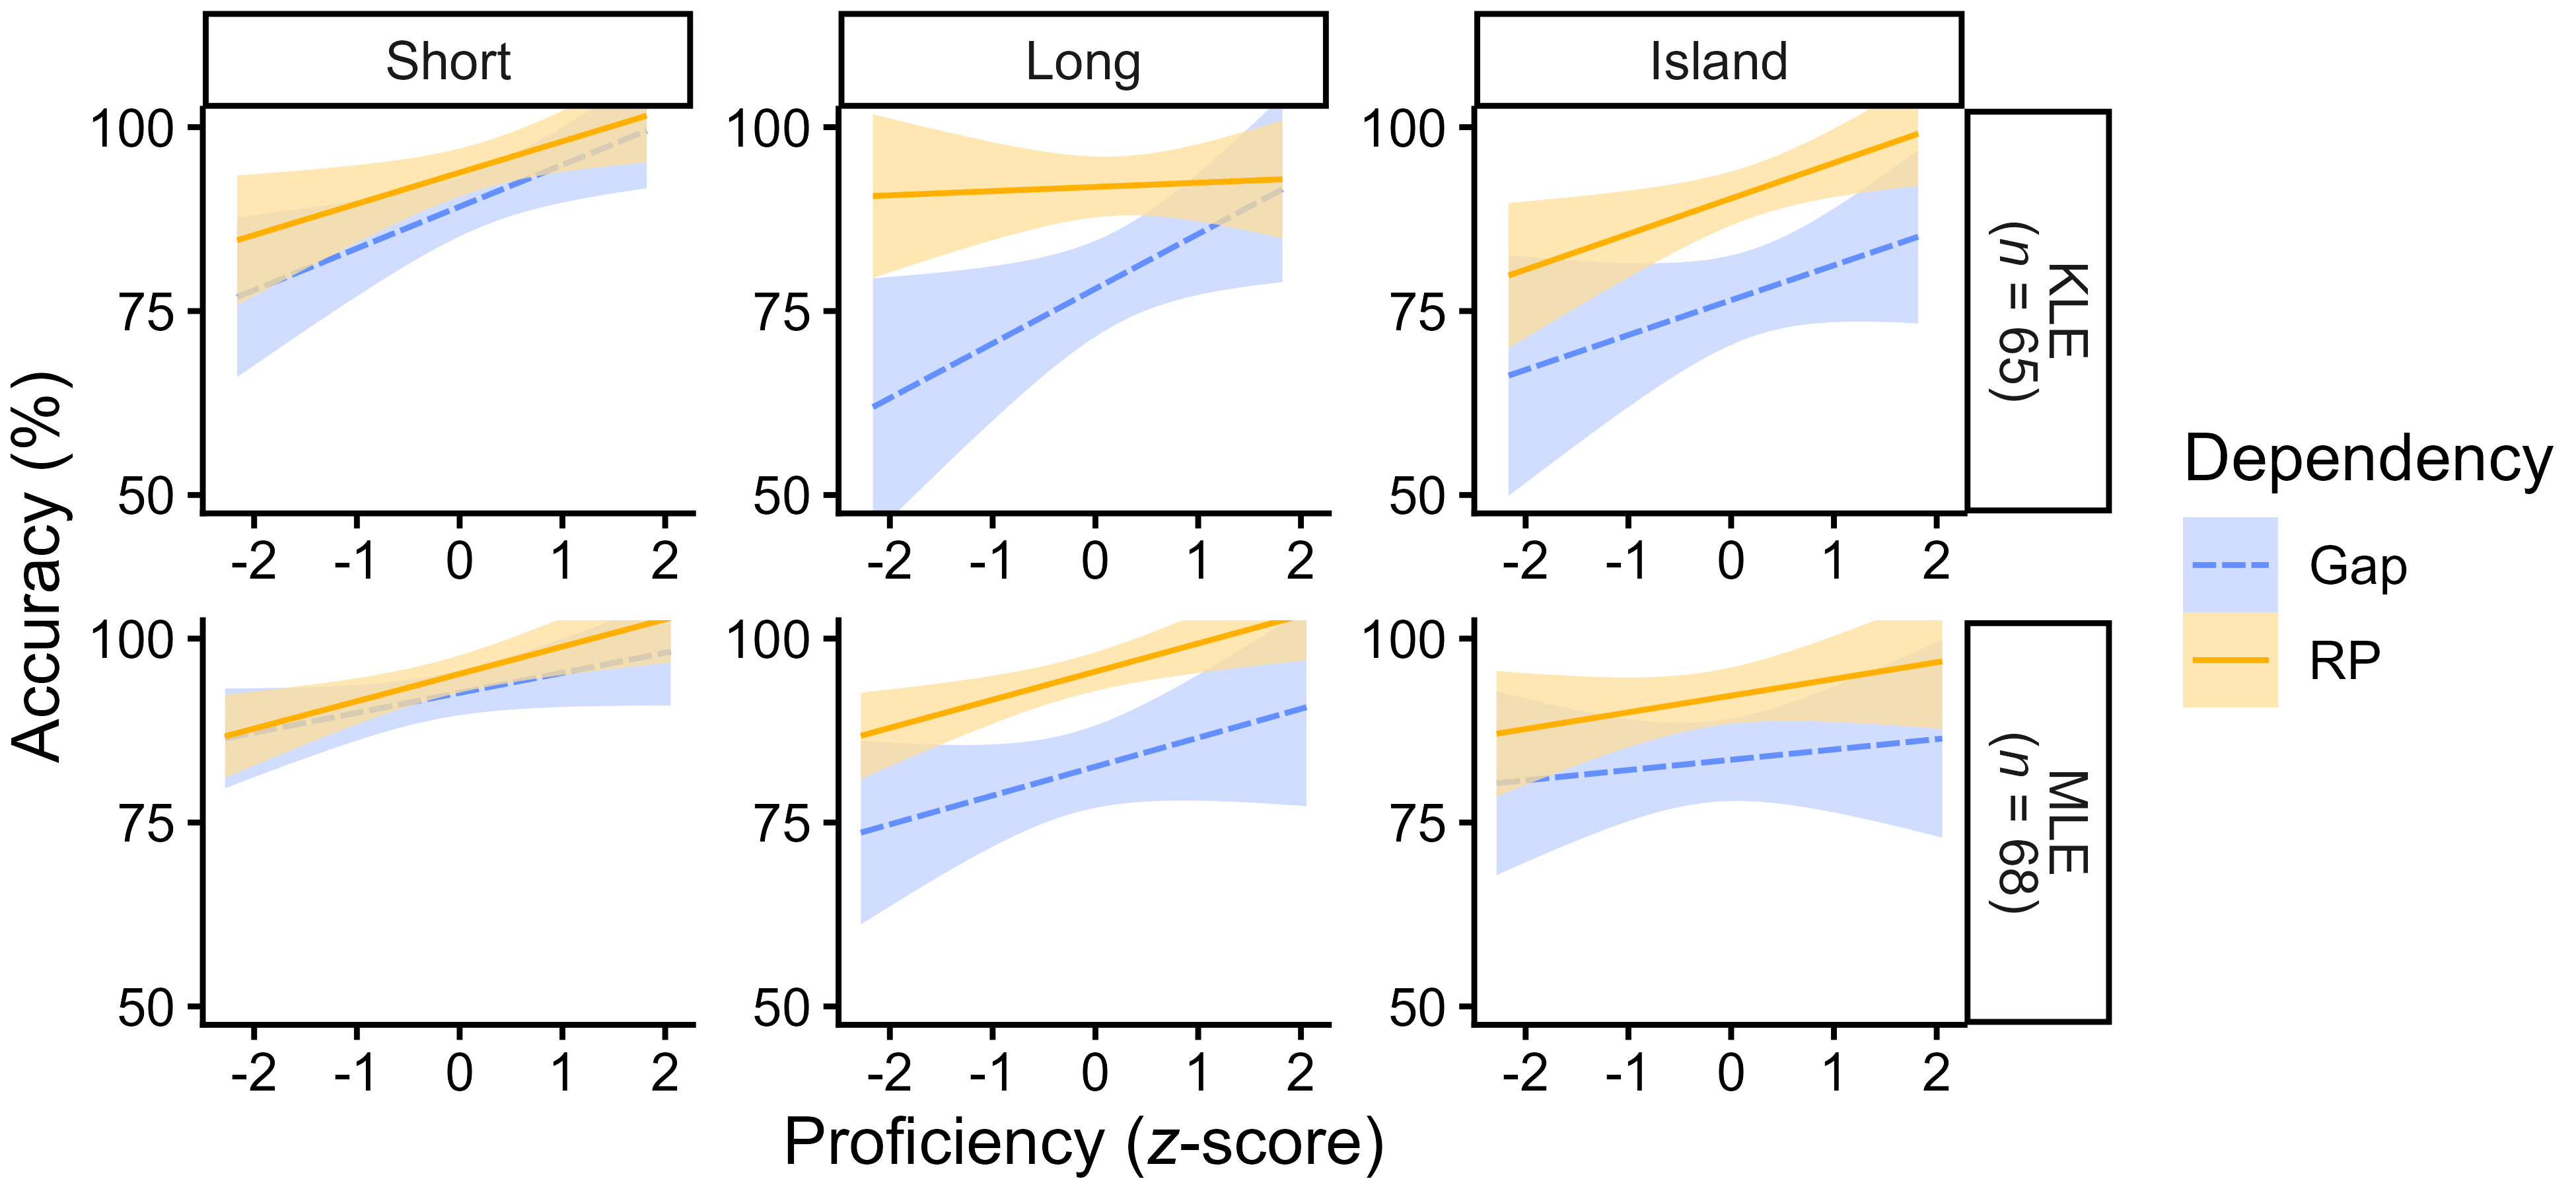
\includegraphics[width=\textwidth]{../analysis/plots/src_spr_accuracy_proficiency.png}
\textit{Note}. Shading indicates 95\% \textit{CI}s.
\vspace{-12pt}
\end{figure}

\noindent The slopes of the regression lines are positive for each combination of \textsc{dependency}, \textsc{environment}, and \textsc{group}, suggesting that accuracy rates tended to rise as proficiency increased. However, it is not evident that there are any strong \textsc{dependency × environment} interactions in the plots, except perhaps for KLEs in the SRC Long condition, where gap-trial accuracy increased more rapidly with rising proficiency than RP-trial accuracy did, such that the size of the RP-over-gap advantage shrank as proficiency scores rose. Weaker versions of the same effect can be seen for several other \textsc{environment} × \textsc{group} combinations, especially in the ORC dataset.

I further probed for proficiency effects in the comprehension-question accuracy data by refitting the mixed-effects logistic regression models for the ORC data and the SRC data separately with \textsc{proficiency} added as a continuous fixed effect. 

The ORC model (model formula: \textsc{accuracy \~{} dependency * environment * group * proficiency + (1 + dependency + environment | participant) + (1 + dependency + environment + group | item)}---see Appendix~\ref{app-results-spr}, Table~\ref{tab:app-orc-spr-accuracy-proficiency-model} for details) found a significant positive relationship between \textsc{accuracy} and \textsc{proficiency} ($\hat{\beta}$~=~0.72, \textit{SE}~=~0.12, $p$~<~.001): As L2 proficiency increased, accuracy increased as well. However, the two-way \textsc{dependency × proficiency} interaction did not come out as significant ($\hat{\beta}$~=~−0.04, \textit{SE}~=~0.12, $p$~=~.758). The three-way \textsc{environment} × \textsc{group} × \textsc{proficiency} interactions were in the marginal-to-significant range, but post-hoc testing did not find the proficiency trend for the [RP~−~gap] contrast to be significant for any combination of \textsc{environment} and \textsc{group}.

The SRC model (model formula: \textsc{accuracy \~{} dependency * environment * group * proficiency + (1 + dependency | participant) + (1 + dependency + group | item)}---see Appendix~\ref{app-results-spr}, Table~\ref{tab:app-src-spr-accuracy-proficiency-model} for details) yielded a significant effect of \textsc{proficiency}, with accuracy rates tending to rise as proficiency increased ($\hat{\beta}$~=~0.51, \textit{SE}~=~0.12, $p$~<~.001). Once again, the two-way \textsc{dependency × proficiency} interaction was not found to be significant ($\hat{\beta}$~=~0.20, \textit{SE}~=~0.13, $p$~=~.120), indicating that the size of the [RP~−~gap] contrast did not vary in a statistically meaningful way across proficiency scores. None of the interactions involving \textsc{dependency}, \textsc{environment}, and \textsc{group} approached significance, suggesting that the proficiency trend for the [RP~−~gap] contrast was not significant for any of the \textsc{environment} × \textsc{group} combinations individually, either.

These results indicate that while overall accuracy on comprehension questions increased with rising L2 English proficiency, particularly in the ORC dataset, the size of the RP-over-gap advantage in accuracy rates was not influenced by proficiency to a statistically meaningful extent.

%========================================================%
\section{Comprehension-question RTs}\label{spr-qrt}
%========================================================%

To address RQ3, I examined the amount of time it took for participants to read and respond to the comprehension questions (starting from when the question appeared on the computer screen). Figures \ref{fig:spr-question-logrt-orc} and \ref{fig:spr-question-logrt-src} show the mean log RTs for comprehension questions in, respectively, the ORC data and the SRC data. Plots of the raw RT data, which displayed the same general pattern of results, are provided in Appendix~\ref{app-results-spr}, Figures~\ref{fig:app-orc-spr-question-rt} and \ref{fig:app-src-spr-question-rt}.

\begin{figure}
\caption{Mean log RTs for comprehension questions in the ORC self-paced reading task} \label{fig:spr-question-logrt-orc}
\raggedright\setstretch{1}
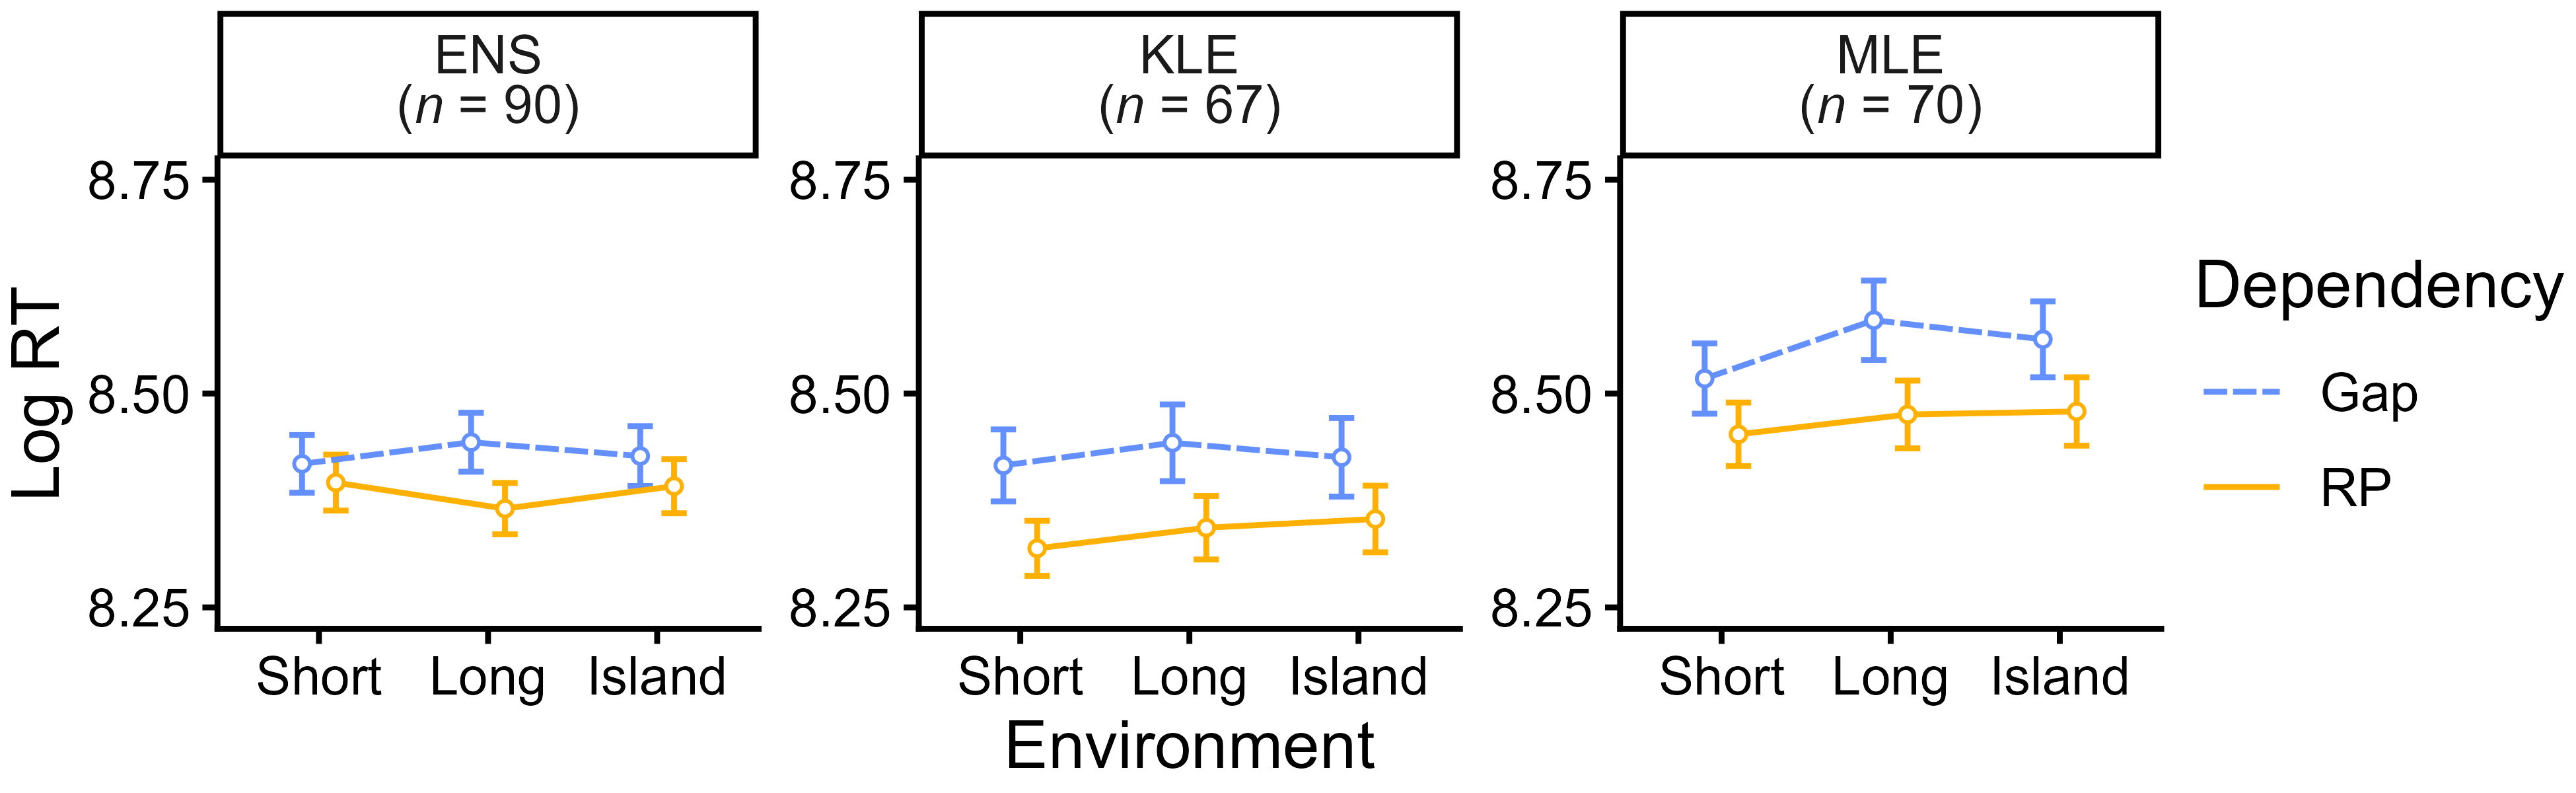
\includegraphics[width=\textwidth]{../analysis/plots/orc_spr_question_logrt_overall.png}
\textit{Note}. Error bars are 95\% \textit{CI}s.
\vspace{-12pt}
\end{figure}

\begin{figure}
\caption{Mean log RTs for comprehension questions in the SRC self-paced reading task} \label{fig:spr-question-logrt-src}
\raggedright\setstretch{1}
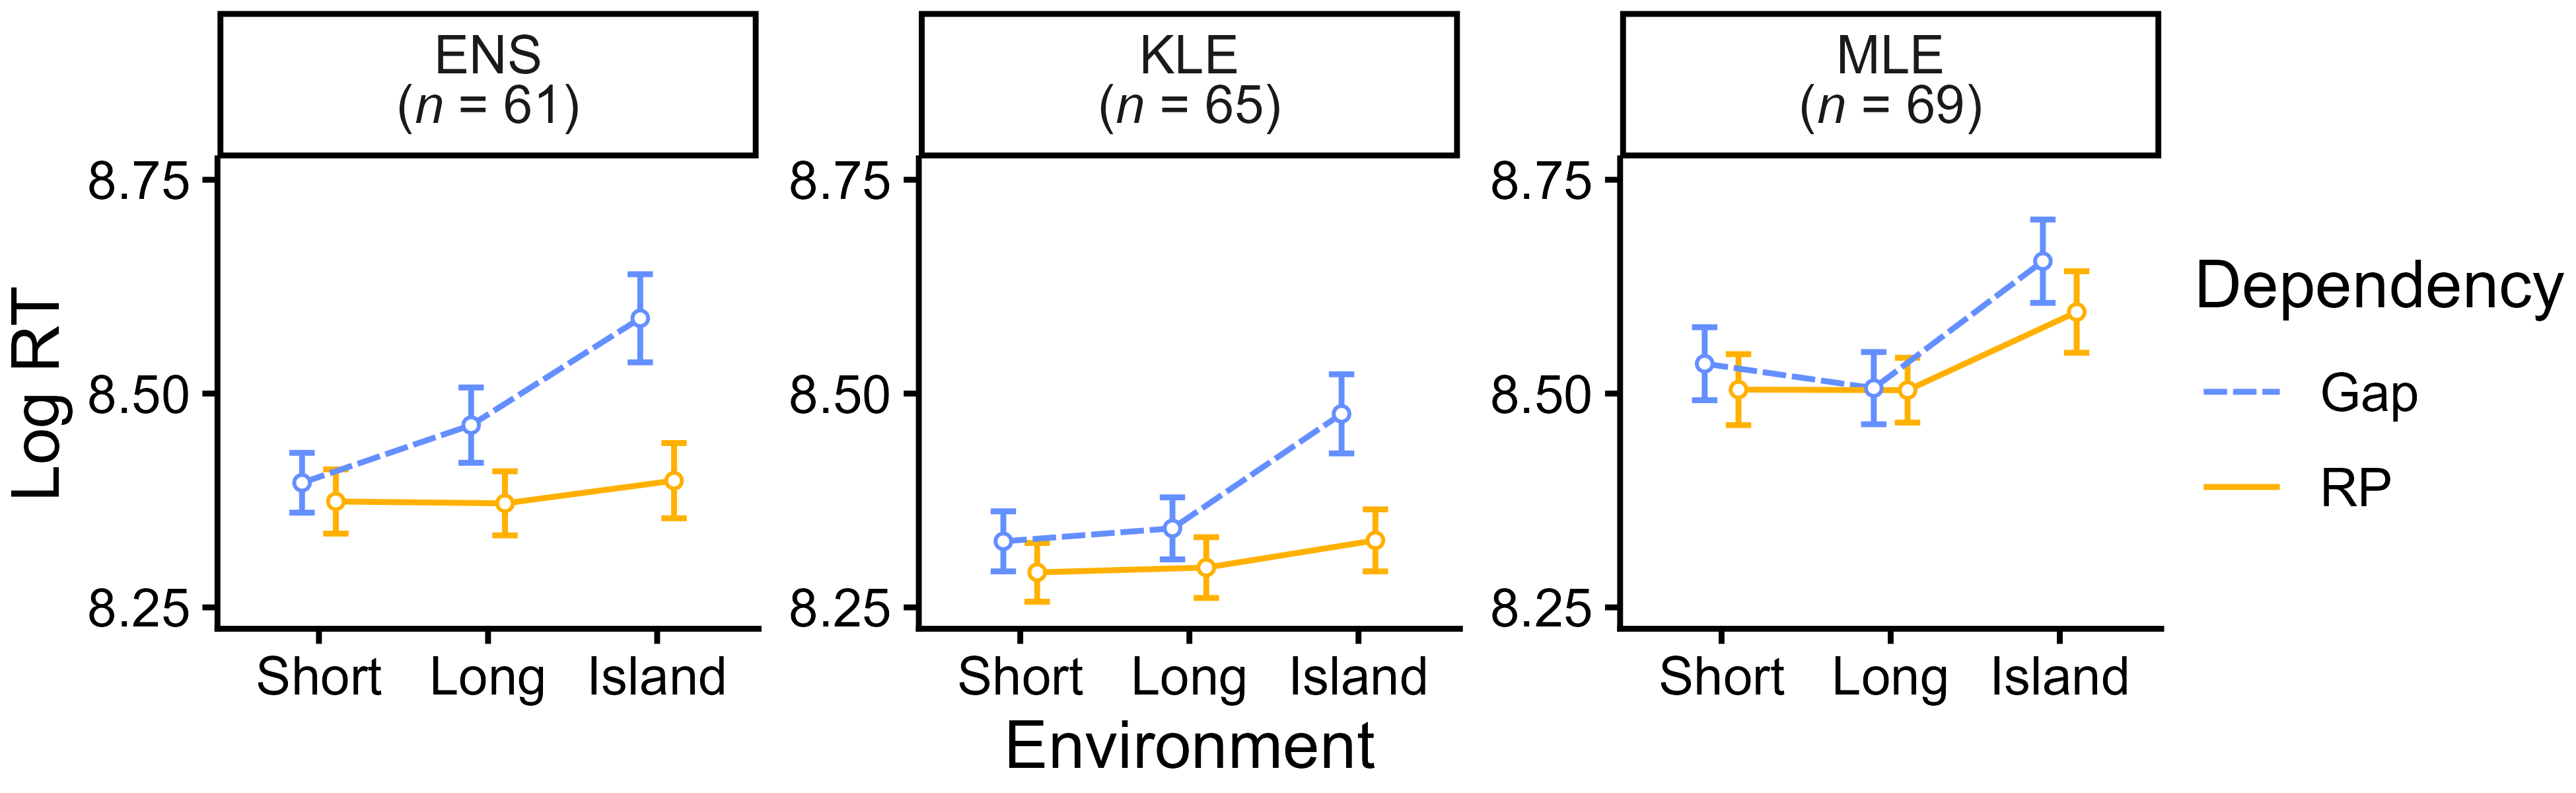
\includegraphics[width=\textwidth]{../analysis/plots/src_spr_question_logrt_overall.png}
\textit{Note}. Error bars are 95\% \textit{CI}s.
\vspace{-12pt}
\end{figure}

\noindent Like in the comprehension-question accuracy data, there was a numerical advantage for RPs relative to gaps for all combinations of \textsc{environment} and \textsc{group}. That is to say, RP-trial responses were, on average, faster than gap-trial responses. The magnitude of the RP advantage did not vary much across conditions in the ORC dataset, but it increased down the SLW hierarchy in the SRC dataset such that the contrast was larger in the Island condition than in the Short and Long conditions.

I examined these patterns further by fitting the log RTs from the ORC and SRC datasets to separate linear mixed-effects regression models. 

The ORC model (model formula: \textsc{log rt \~{} dependency * environment * group + (1 + dependency + environment | participant) + (1 + dependency + environment + group | item)}---see Appendix~\ref{app-results-spr}, Table~\ref{tblr:app-orc-spr-question-logrt-model} for details) found significant effects for (a)~\textsc{dependency}, with RP trials having faster RTs than gap trials ($\hat{\beta}$~=~−0.08, \textit{SE}~=~0.01, $p$~<~.001), (b)~\textsc{environment}, with Long-condition trials and Island-condition trials both having slower RTs than Short-condition trials (Long~−~Short: $\hat{\beta}$~=~0.02, \textit{SE}~=~0.01, $p$~=~.029; Island~−~Short: $\hat{\beta}$~=~0.02, \textit{SE}~=~0.01, $p$~=~.046), and (c)~\textsc{group}, with MLEs having slower RTs than ENSs ($\hat{\beta}$~=~0.10, \textit{SE}~=~0.04, $p$~=~.011). Several of the two-way interactions involving \textsc{dependency}, \textsc{environment}, and \textsc{group} also came out as significant. In the pairwise comparisons, the [RP~−~gap] contrast was found to be significant for ENSs only in the Long condition ($\hat{\beta}$~=~−0.08, \textit{SE}~=~0.02, $p$~=~.003); for KLEs and MLEs, though, the contrast came out as significant in all three environments (all $p$s~<~.05).

The SRC model (model formula: \textsc{log rt \~{} dependency * environment * group + (1 + dependency + environment | participant) + (1 + dependency + environment + group | item)}---see Appendix~\ref{app-results-spr}, Table~\ref{tblr:app-src-spr-question-logrt-model} for details) found significant effects for (a)~\textsc{dependency}, with RP trials having faster RTs than gap trials ($\hat{\beta}$~=~−0.07, \textit{SE}~=~0.01, $p$~<~.001), (b)~\textsc{environment}, with the Island condition having slower RTs than the Short condition (Island~−~Short: $\hat{\beta}$~=~0.11, \textit{SE}~=~0.01, $p$~<~.001), and (c)~\textsc{group}, with KLEs having faster RTs than ENSs ($\hat{\beta}$~=~−0.10, \textit{SE}~=~0.04, $p$~=~.018) but MLEs having slower RTs than ENSs ($\hat{\beta}$~=~0.12, \textit{SE}~=~0.04, $p$~=~.005). Several of the two-way and three-way interactions also came out as significant ($p$~<~.05). In the pairwise comparisons, the [RP~−~gap] contrast was found to be significant for ENSs in the Long and Island conditions (Long: $\hat{\beta}$~=~−0.09, \textit{SE}~=~0.03, $p$~=~.002; Island: $\hat{\beta}$~=~−0.20, \textit{SE}~=~0.03, $p$~<~.001); for KLEs and MLEs, the contrast came out as significant only in the Island condition (KLE: $\hat{\beta}$~=~−0.15, \textit{SE}~=~0.02, $p$~<~.001; MLE: $\hat{\beta}$~=~−0.09, \textit{SE}~=~0.02, $p$~=~.004).

To review, an RP-over-gap advantage in comprehension-question RTs was observed across all levels of \textsc{group} and \textsc{environment}, and this contrast rose to the level of significance for each group in the Long and/or Island conditions. The fact that the RP advantage was larger in the SRC Island condition than in the ORC Island condition, at least for ENSs, lends support to the idea that in English, \textit{wh}-island SRCs are stronger islands than \textit{wh}-island ORCs. Overall, these results provide additional corroborating evidence that resumptive RCs ease real-time comprehension of RCs under high cognitive load. 

%========================================================%
\section{L2 proficiency effects for comprehension-question RTs}\label{spr-qrt-proficiency}
%========================================================%

Lastly, let us examine how L2 proficiency related to comprehension-question RTs. Figures \ref{fig:spr-question-logrt-proficiency-orc} and \ref{fig:spr-question-logrt-proficiency-src} show the relationship between L2 proficiency scores and log RTs for, respectively, the ORC data and the SRC data. There was a general tendency for RTs to get faster with growing proficiency, except for MLEs in the SRC dataset, whose RTs appeared to get slightly slower as proficiency scores went up. However, it is not evident that there are any strong \textsc{dependency} × \textsc{proficiency} interactions in the plots for any of the \textsc{environment} × \textsc{group} combinations.

\begin{figure}
\caption{Relationship between L2 proficiency and comprehension-question RTs in the ORC self-paced reading task} \label{fig:spr-question-logrt-proficiency-orc}
\raggedright\setstretch{1}
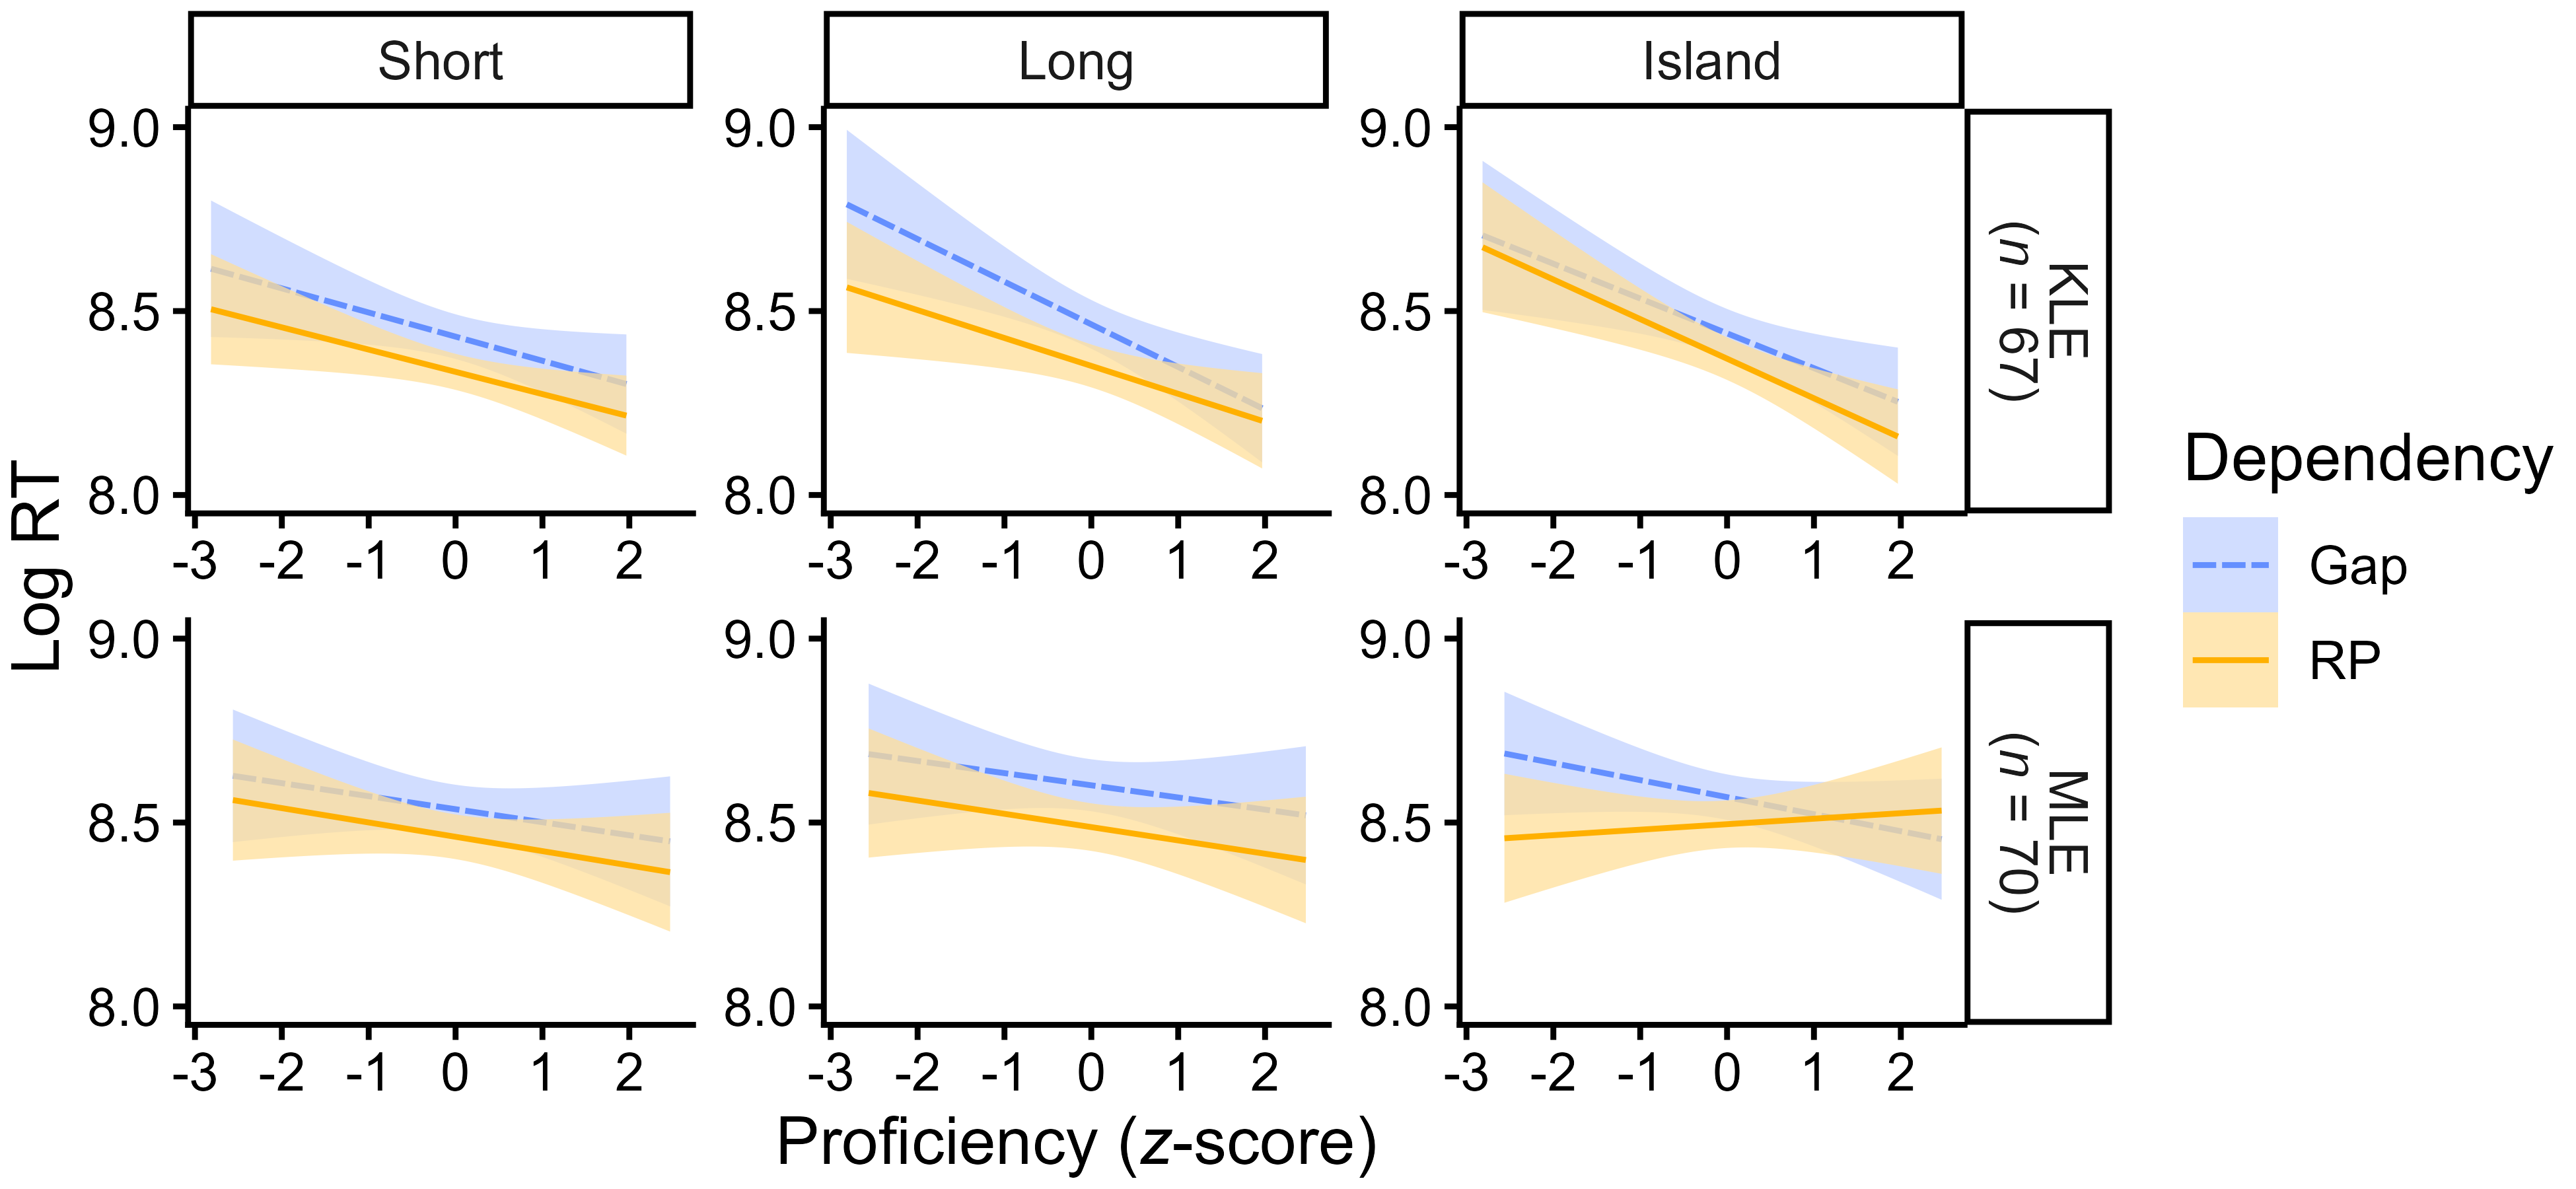
\includegraphics[width=\textwidth]{../analysis/plots/orc_spr_question_logrt_proficiency.png}
\textit{Note}. Shading indicates 95\% \textit{CI}s.
\vspace{-12pt}
\end{figure}

\begin{figure}
\caption{Relationship between L2 proficiency and comprehension-question RTs in the SRC self-paced reading task} \label{fig:spr-question-logrt-proficiency-src}
\raggedright\setstretch{1}
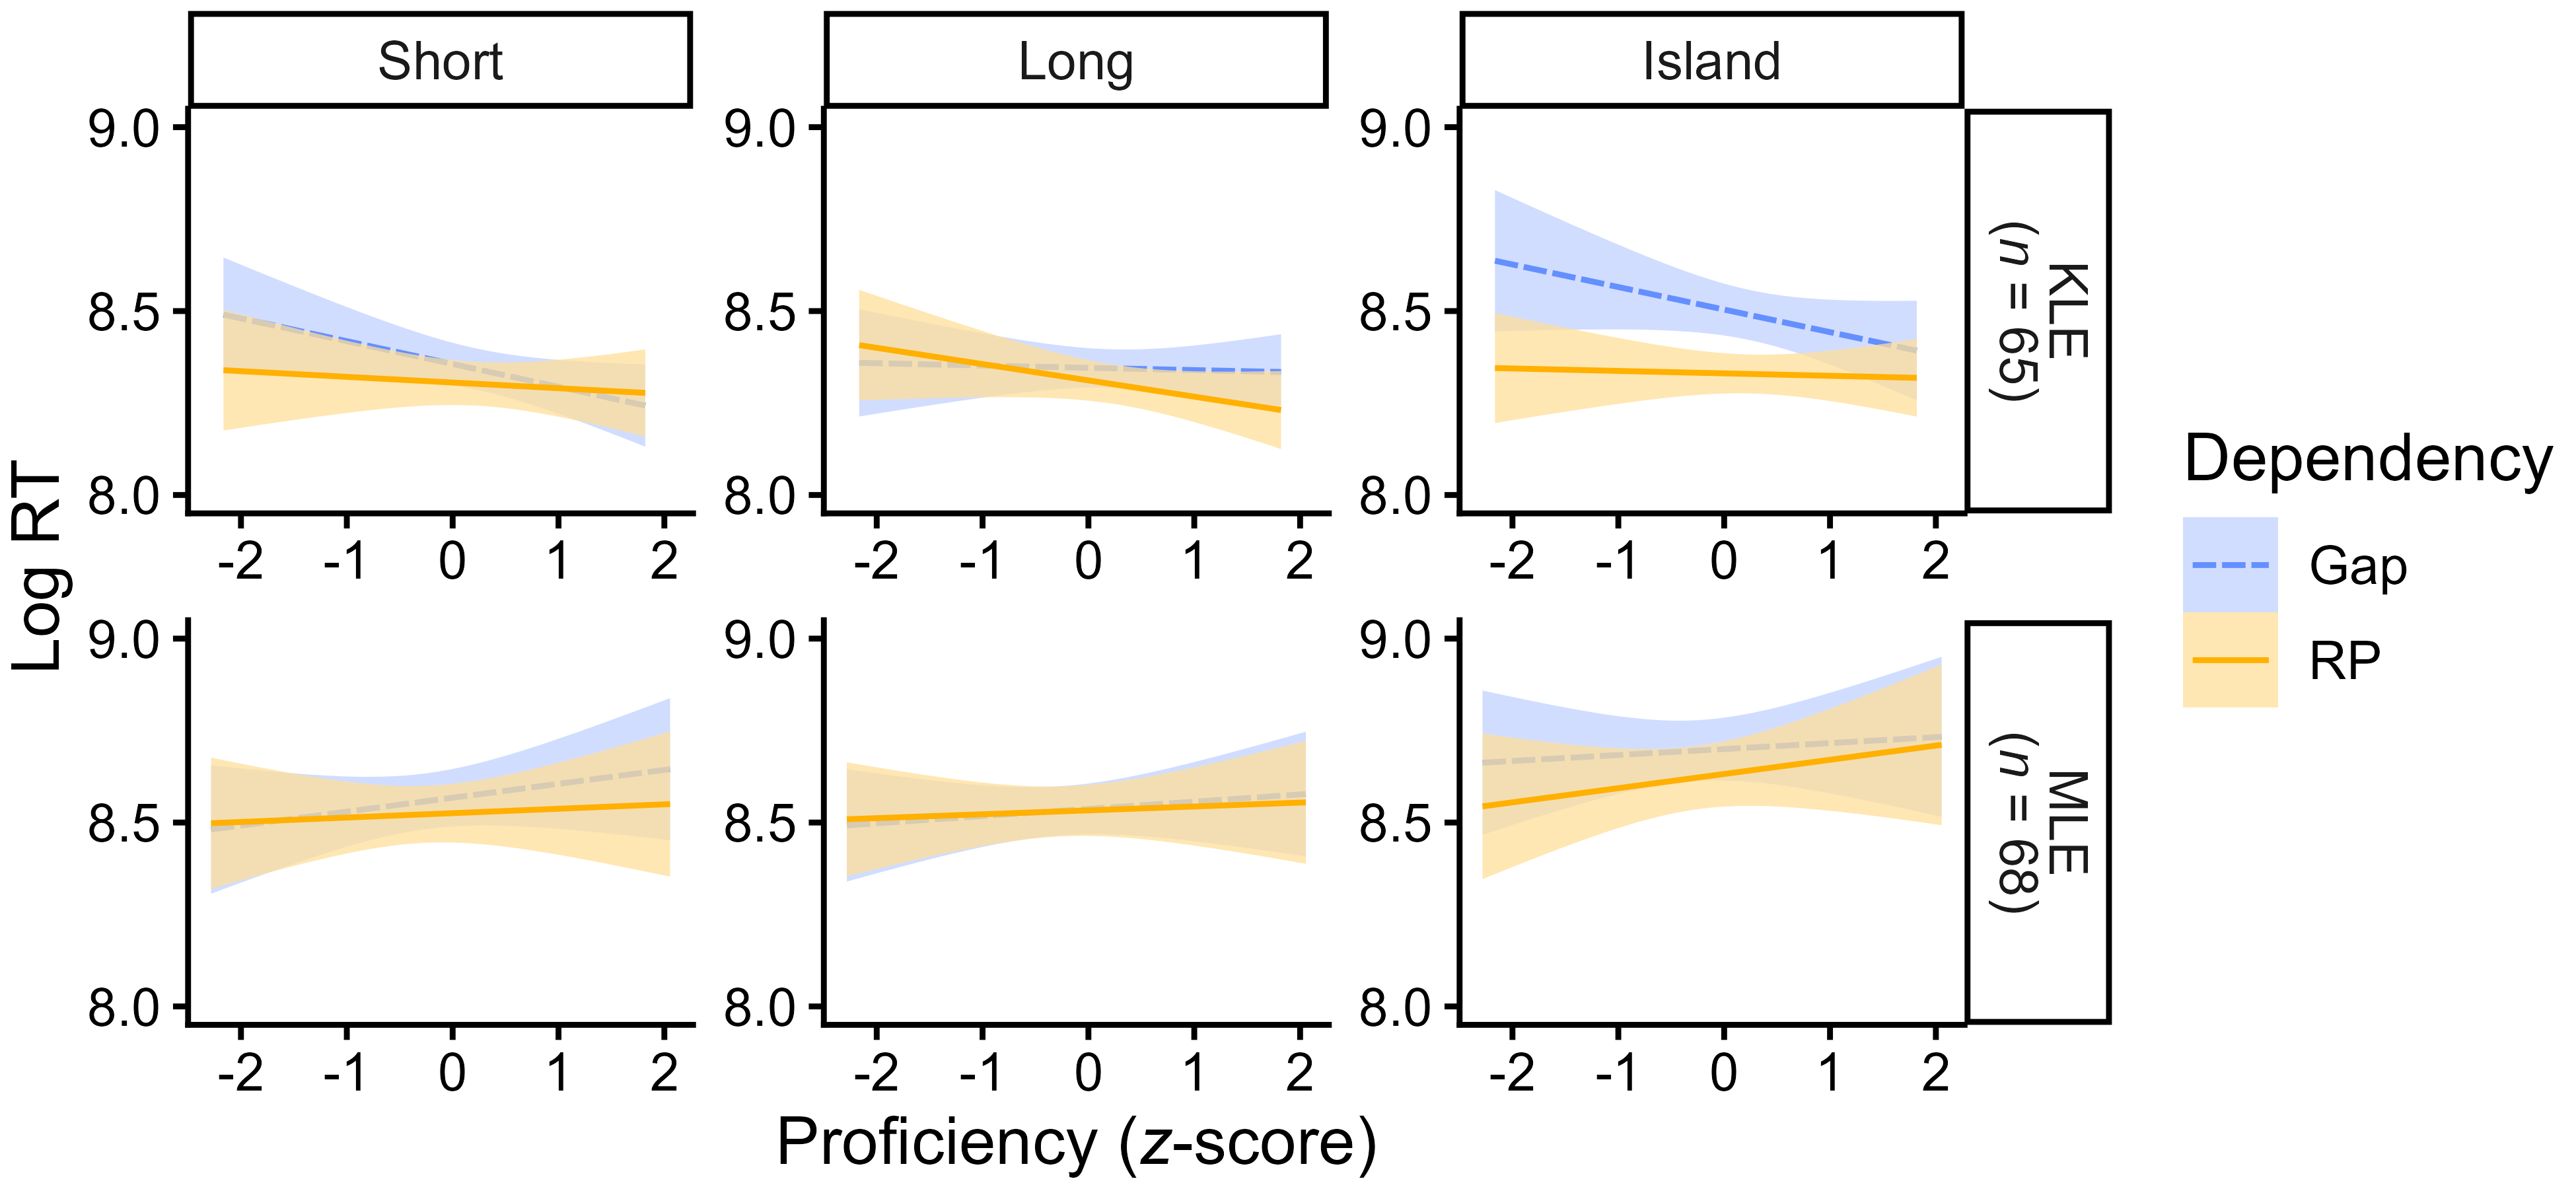
\includegraphics[width=\textwidth]{../analysis/plots/src_spr_question_logrt_proficiency.png}
\textit{Note}. Shading indicates 95\% \textit{CI}s.
\vspace{-12pt}
\end{figure}

As a further test for proficiency effects in the comprehension-question RT data, I refit the linear mixed-effects models for the ORC data and the SRC data separately with \textsc{proficiency} added as a continuous fixed effect. 

The ORC model (model formula: \textsc{log rt \~{} dependency * environment * group * proficiency + (1 + dependency + environment | participant) + (1 + dependency + environment | item)}---see Appendix~\ref{app-results-spr}, Table~\ref{tblr:app-orc-spr-question-logrt-proficiency-model} for details) yielded a significant effect for \textsc{proficiency}, with RTs tending to get faster as proficiency rose ($\hat{\beta}$~=~−0.06, \textit{SE}~=~0.02, $p$~=~.002). However, the \textsc{dependency} × \textsc{proficiency} interaction did not come out as significant ($p$~=~.116), signaling that the [RP~−~gap] contrast did not vary in a statistically meaningful way across the proficiency spectrum. Two of the three-way and four-way interactions involving \textsc{environment}, \textsc{group}, and \textsc{proficiency} were found to be marginally significant, but post-hoc tests revealed that the proficiency trend for the [RP~−~gap] contrast only rose to the level of marginal significance, and only for MLEs in the Island condition ($\hat{\beta}$~=~0.06, \textit{SE}~=~0.02, $p$~=~.085).

The SRC model (model formula: \textsc{log rt \~{} dependency * environment * group * proficiency + (1 + dependency * environment | participant) + (1 | item)}---see Appendix~\ref{app-results-spr}, Table~\ref{tblr:app-src-spr-question-logrt-proficiency-model} for details) found no significant effect for \textsc{proficiency} ($p$~=~.898). The \textsc{dependency × proficiency} interaction did not come out as significant, either ($p$~=~.647), indicating once again that the [RP~−~gap] contrast did not vary significantly across proficiency scores. None of the three-way or four-way interactions involving \textsc{environment}, \textsc{group}, and \textsc{proficiency} approached significance, which suggests that the proficiency trend for the [RP~−~gap] contrast also failed to reach significance for any of the \textsc{environment} × \textsc{group} combinations individually.

These results show that while higher L2 English proficiency was associated with faster overall RTs (at least in the ORC data), the contrast between gap-trial RTs and RP-trial RTs was not strongly affected by the proficiency scores.

%========================================================%
\section{Summing up}\label{spr-conclusion}
%========================================================%

This chapter has provided robust evidence that resumption facilitates real-time comprehension of difficult-to-process RCs, contra claims made by advocates of the selfish-speaker model (\cite{ferreira.swets2005,morgan.etal2020,polinsky.etal2013}; see~Section~\ref{res-selfish}) that resumption only helps with language production. Data triangulated from three different sources---region-of-interest RTs, comprehension-question accuracy scores, and comprehension-question RTs---all point towards resumption conferring a processing advantage over gapping at lower levels on the SLW hierarchy. Proficiency effects were also observed whereby RTs tended to be faster and accuracy tended to be higher for L2ers with more advanced English proficiency. This suggests that, unsurprisingly, L2ers grow more efficient at parsing RCs as their proficiency increases. However, the [RT~−~gap] contrasts in RTs and in accuracy scores were not found to be strongly affected by proficiency in the analyses reported in this chapter.  What remains to be seen is how these processing effects relate to perceptions of well-formedness (see~Chapter~\ref{ch-reanalysis}). To begin tackling that question, I pivot in the next chapter to examining the acceptability judgment data.